\setcounter{section}{2}
\section{从溶液中生长晶体的方法}
从溶液中生长晶体过程的最关键因素是控制溶液的过饱和度。使溶液达到过饱和状态,在晶体生长过程中维持其过饱和度的途径有:
\begin{enumerate}[(1)]\itemsep -0.5ex
\item 据溶解度曲线,改变温度。
\item 采取各种方式(如蒸发、电解)移去溶剂,改变溶液成分。
\item 通过化学反应来控制过饱和度。由于化学反应速度和晶体生长速度差别很大,做到这一点是很困难的,需要采取一些特殊的方式,如通过凝胶扩散使反应缓慢进行等。
\item 用亚稳相来控制过饱和度,即利用某些物质的稳定相和亚稳相的溶解度差别,控制一定的温度,使亚稳相不断溶解,稳定相不断生长。
\end{enumerate}

根据晶体的溶解度和温度系数,从溶液中生长晶体的具体方法有下述几种。

\subsection{降温法}
降温法是从溶液中培养晶体的一种最常用的方法。这种方法适用于溶解度和温度系数都较大的物质,并需要一定的温度区间。这一温度区间也是有限制的:温度上限由于蒸发量大而不宜过高,当温度下限太低时,对晶体生长也不利。一般来说,比较合适的起始温度是50---60℃,降温区间以15---20℃为宜。

降温法的基本原理是利用物质较大的正溶解度温度系数,在晶体生长过程中逐渐降低温度,使析出的物质不断在晶体上生长。用这种方法生长的物质的溶解度温度系数最好不低于1.5g/1000g$\text{溶液}\cdot$℃,表3.7列出符合此要求的一些物质的数据。

\begin{table}[h]
\centering
\caption{40℃时,一些物质的溶解度及其温度系数}
\begin{tabular}{c|c|c}\toprule
物质 & \tabincell{c}{溶解度\\(g/1000g溶液)} & \tabincell{c}{溶解度温度系数\\g/1000g$\text{溶液}\cdot$℃}\\\hline
明矾\quad$\rm K_2SO_4\cdot Al_2(SO_4)_3\cdot 24H_2O$ & 240 & $+9.0$\\
ADP\quad$\rm NH_4H_2PO_4$ & 360 & $+4.9$\\
TGS\quad$\rm (NH_2CH_2COOH)_3\cdot H_2SO_4$ & 300 & $+4.6$\\
KDP\quad$\rm KH_2PO_4$ & 250 & $+3.5$\\
EGT\quad$\rm ???$ & 598 & $+2.1$\\
\bottomrule
\end{tabular}
\end{table}

降温法生长晶体的几种装置,如图3.18、图3.19和图3.20所示。

在降温法生长晶体的整个过程中,必须严格控制温度,并按一定程序降温。研究表明,微小的温度波动就足以在生长的晶体中造成某些不均匀区域。为提高晶体生长的完整性,要求控温精度尽可能高(目前已达±0.001℃),此外还需造成适合晶体生长的其他条件。

\begin{figure}[h]
 \centering
 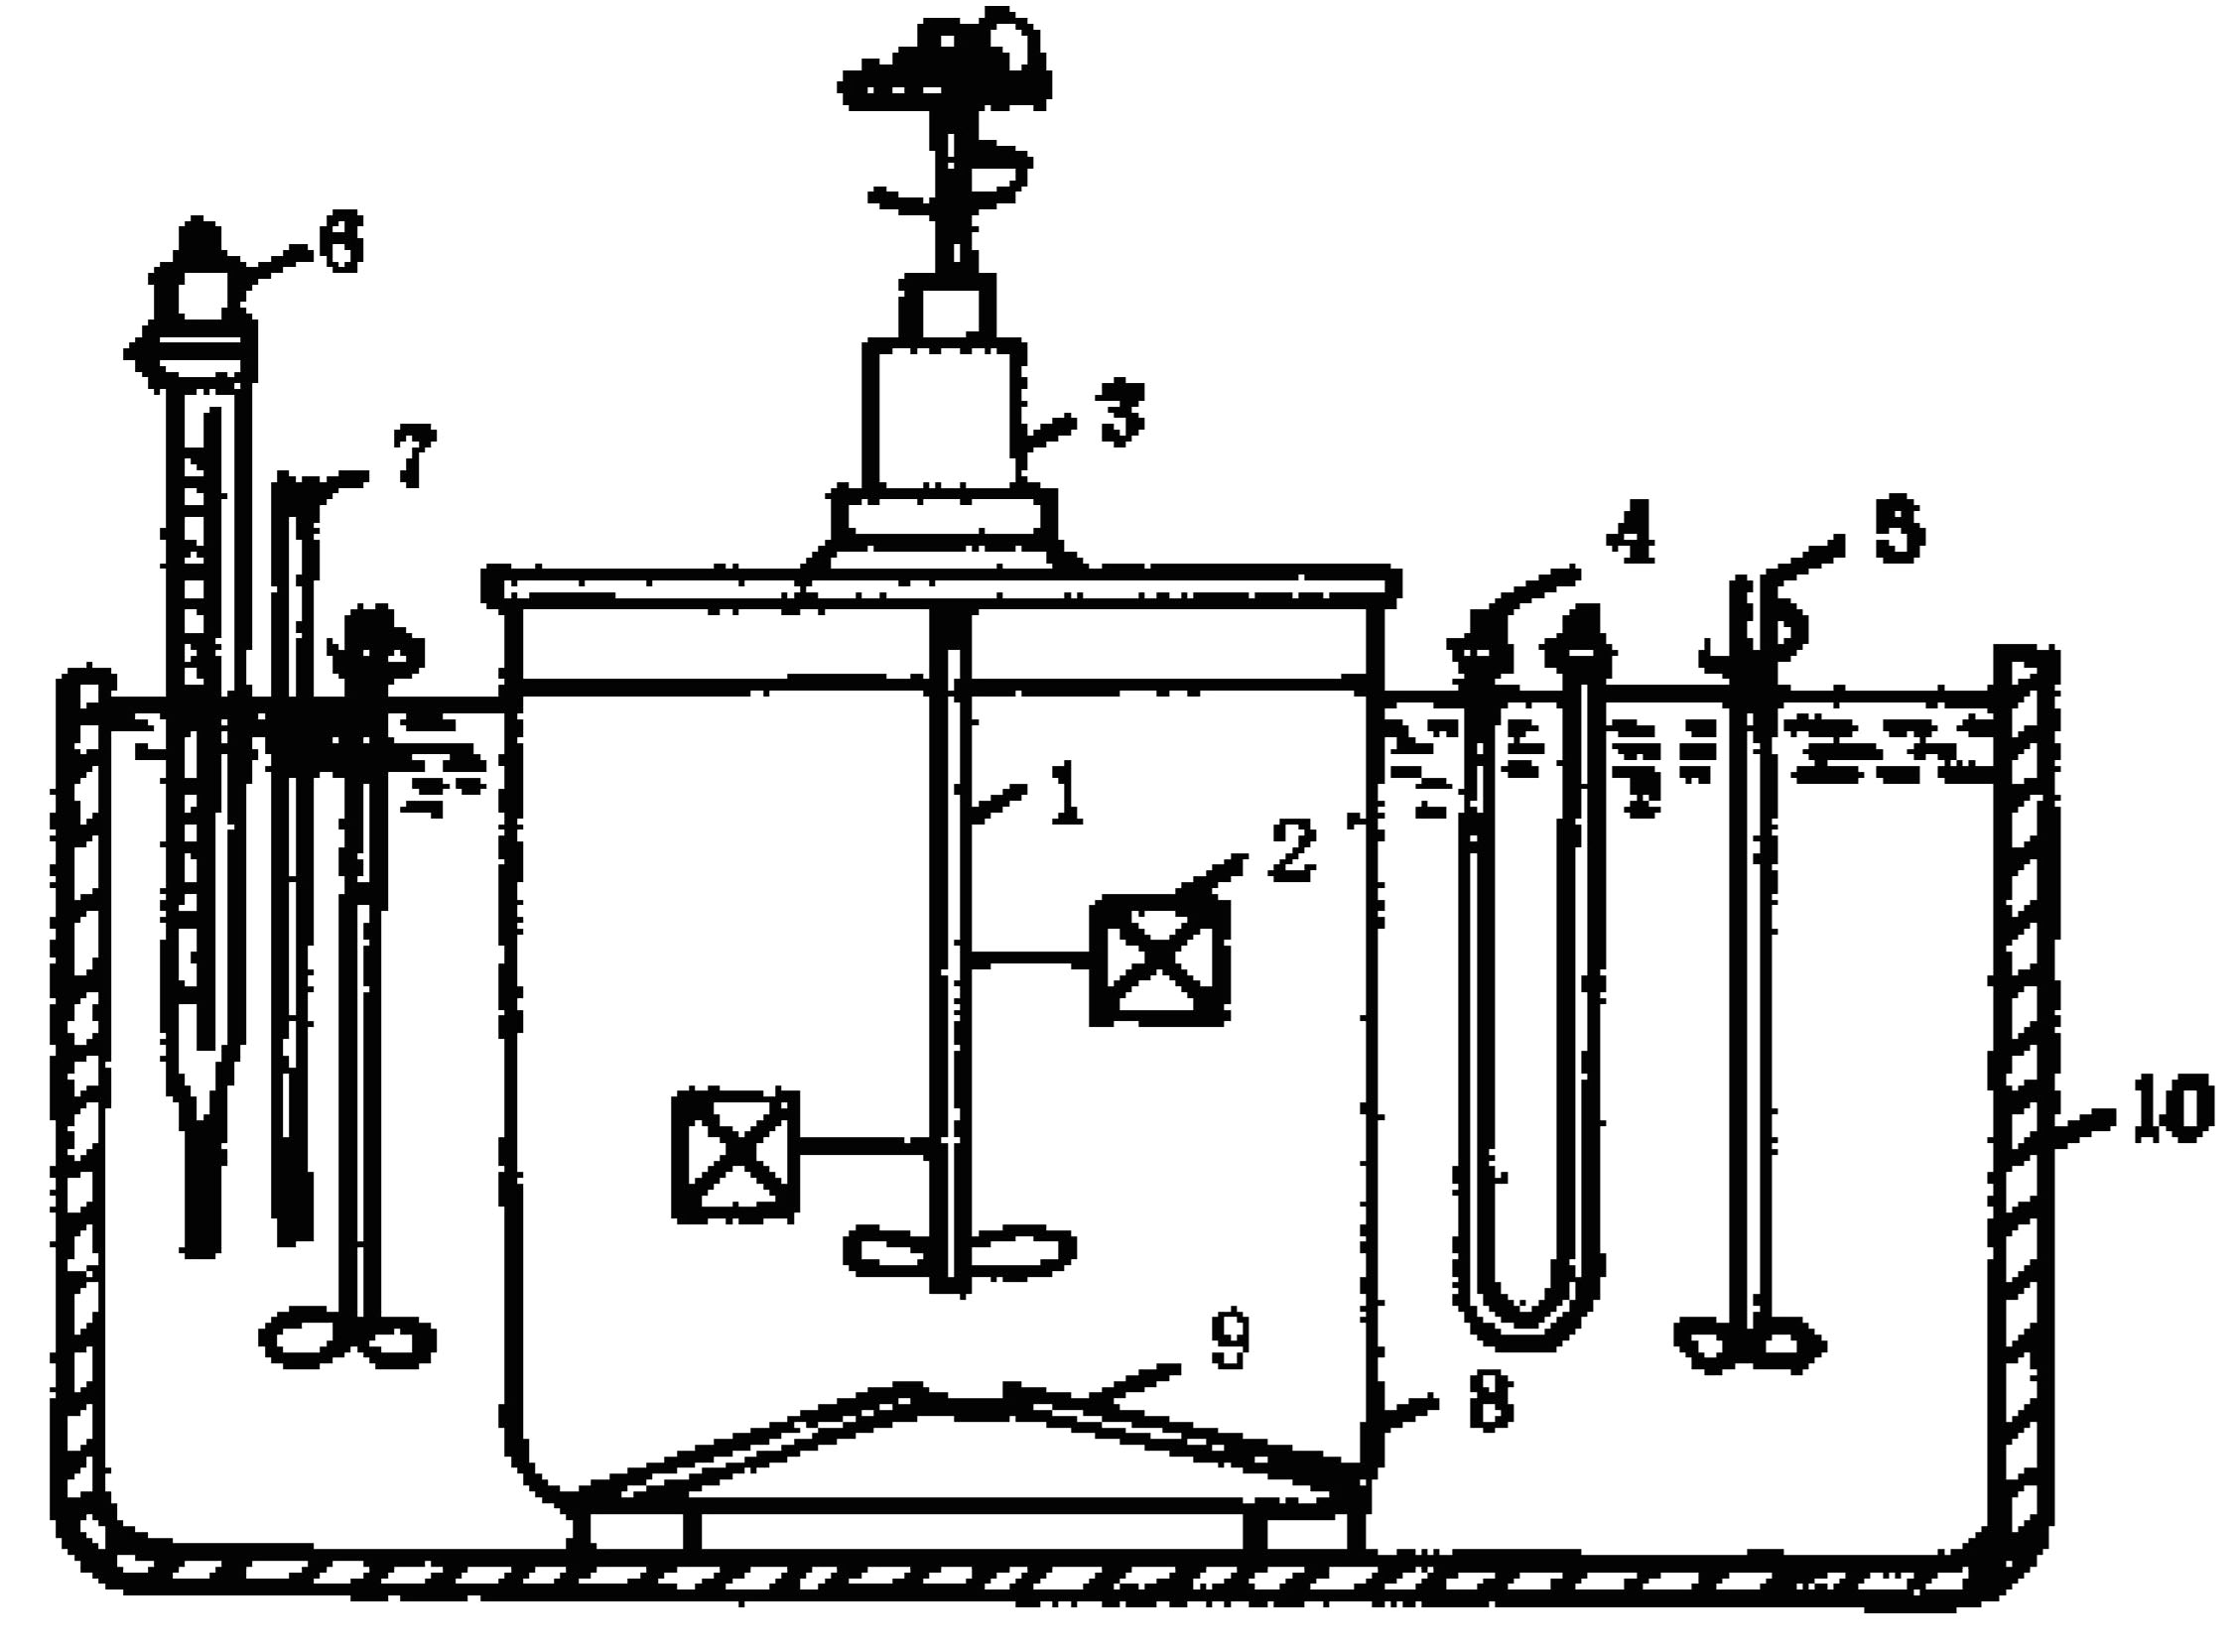
\includegraphics[width=0.5\textwidth]{fig/cp03/img3.18.jpg}
 \caption{水浴育晶装置。图中:}
 1为掣晶杆;2为晶体;3为转动密封装置;4为浸没式加热器; \\
 5为搅拌器;6为控制器(接触温度计);7为温度计;8为育晶器;\\
 9为有孔隔板;10为水槽。
\end{figure}

在利用降温法来生长晶体的过程中可不用再补充溶液或溶质。因此,整个育晶器在生长过程中必须严格密封,以防溶剂蒸发和外界的污染。例如从重水溶液中生长晶体时,如果密封不好,溶液中的D$_2$O就会同大气中的H$_2$O汽发生同位素交换而使溶液氘化程度下降。为增加温度的稳定性,育晶器的容量必须要大些(大型育晶器有几十升至上千升),加热保温方式有水浴槽或内部加热、外壳加保温套等。育晶器顶部经常有保持冷凝水回流,底部有电炉加热为好,使得溶液表面和底部都有不饱和层保护,避免自发晶核形成。

育晶器内的控温精度除了与育晶装置的结构有关外,很大程度上取决于控温装置,继电器开关式控温一般可以满足水溶液晶体生长的要求,温度波动可以控制在±0.05℃以下,用PID控温方式,特别是使用可编程温度控制器控温,实现控温精度至±0.005℃并不困难,这对培养高完整性单晶十分有利。

\begin{figure}[htb]
 \centering
 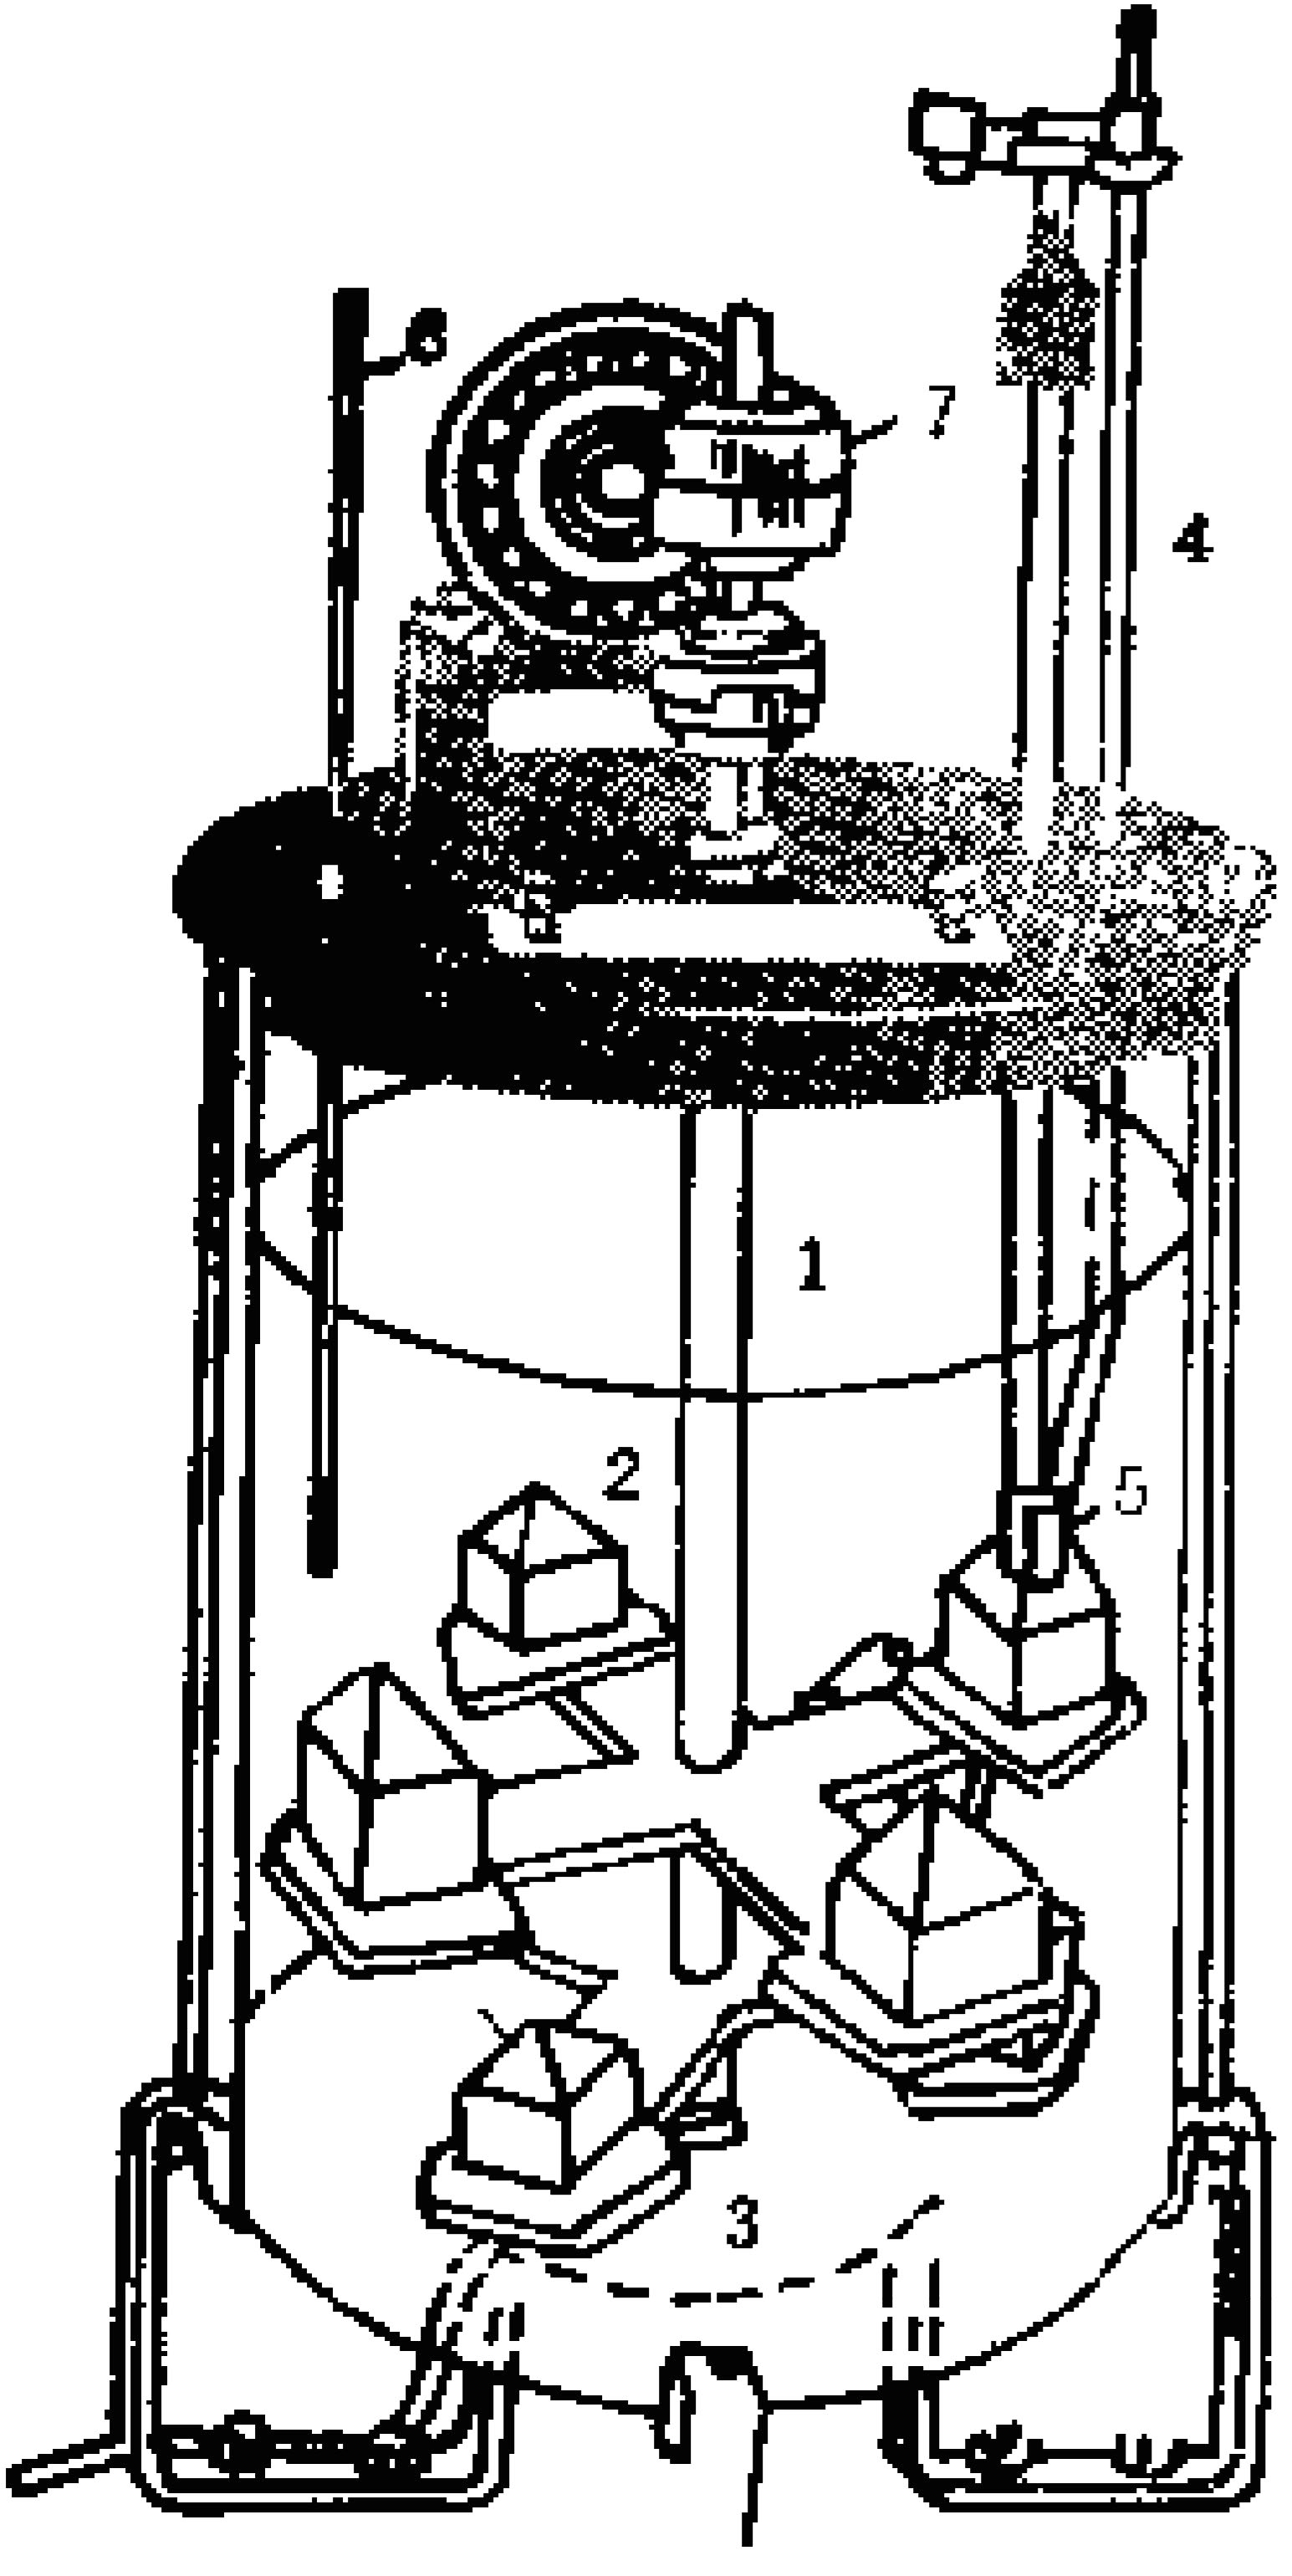
\includegraphics[width=0.3\textwidth]{fig/cp03/img3.19.jpg}
 \caption{直接加热的转动育晶器。}
 图中:1为掣晶板;2为晶体;3为底部主加热器;4为控制器; 5为辅助小灯泡加热器;6为温度计;7为可逆转动装置(30r/min)。
\end{figure}

\begin{figure}[htb]
 \centering
 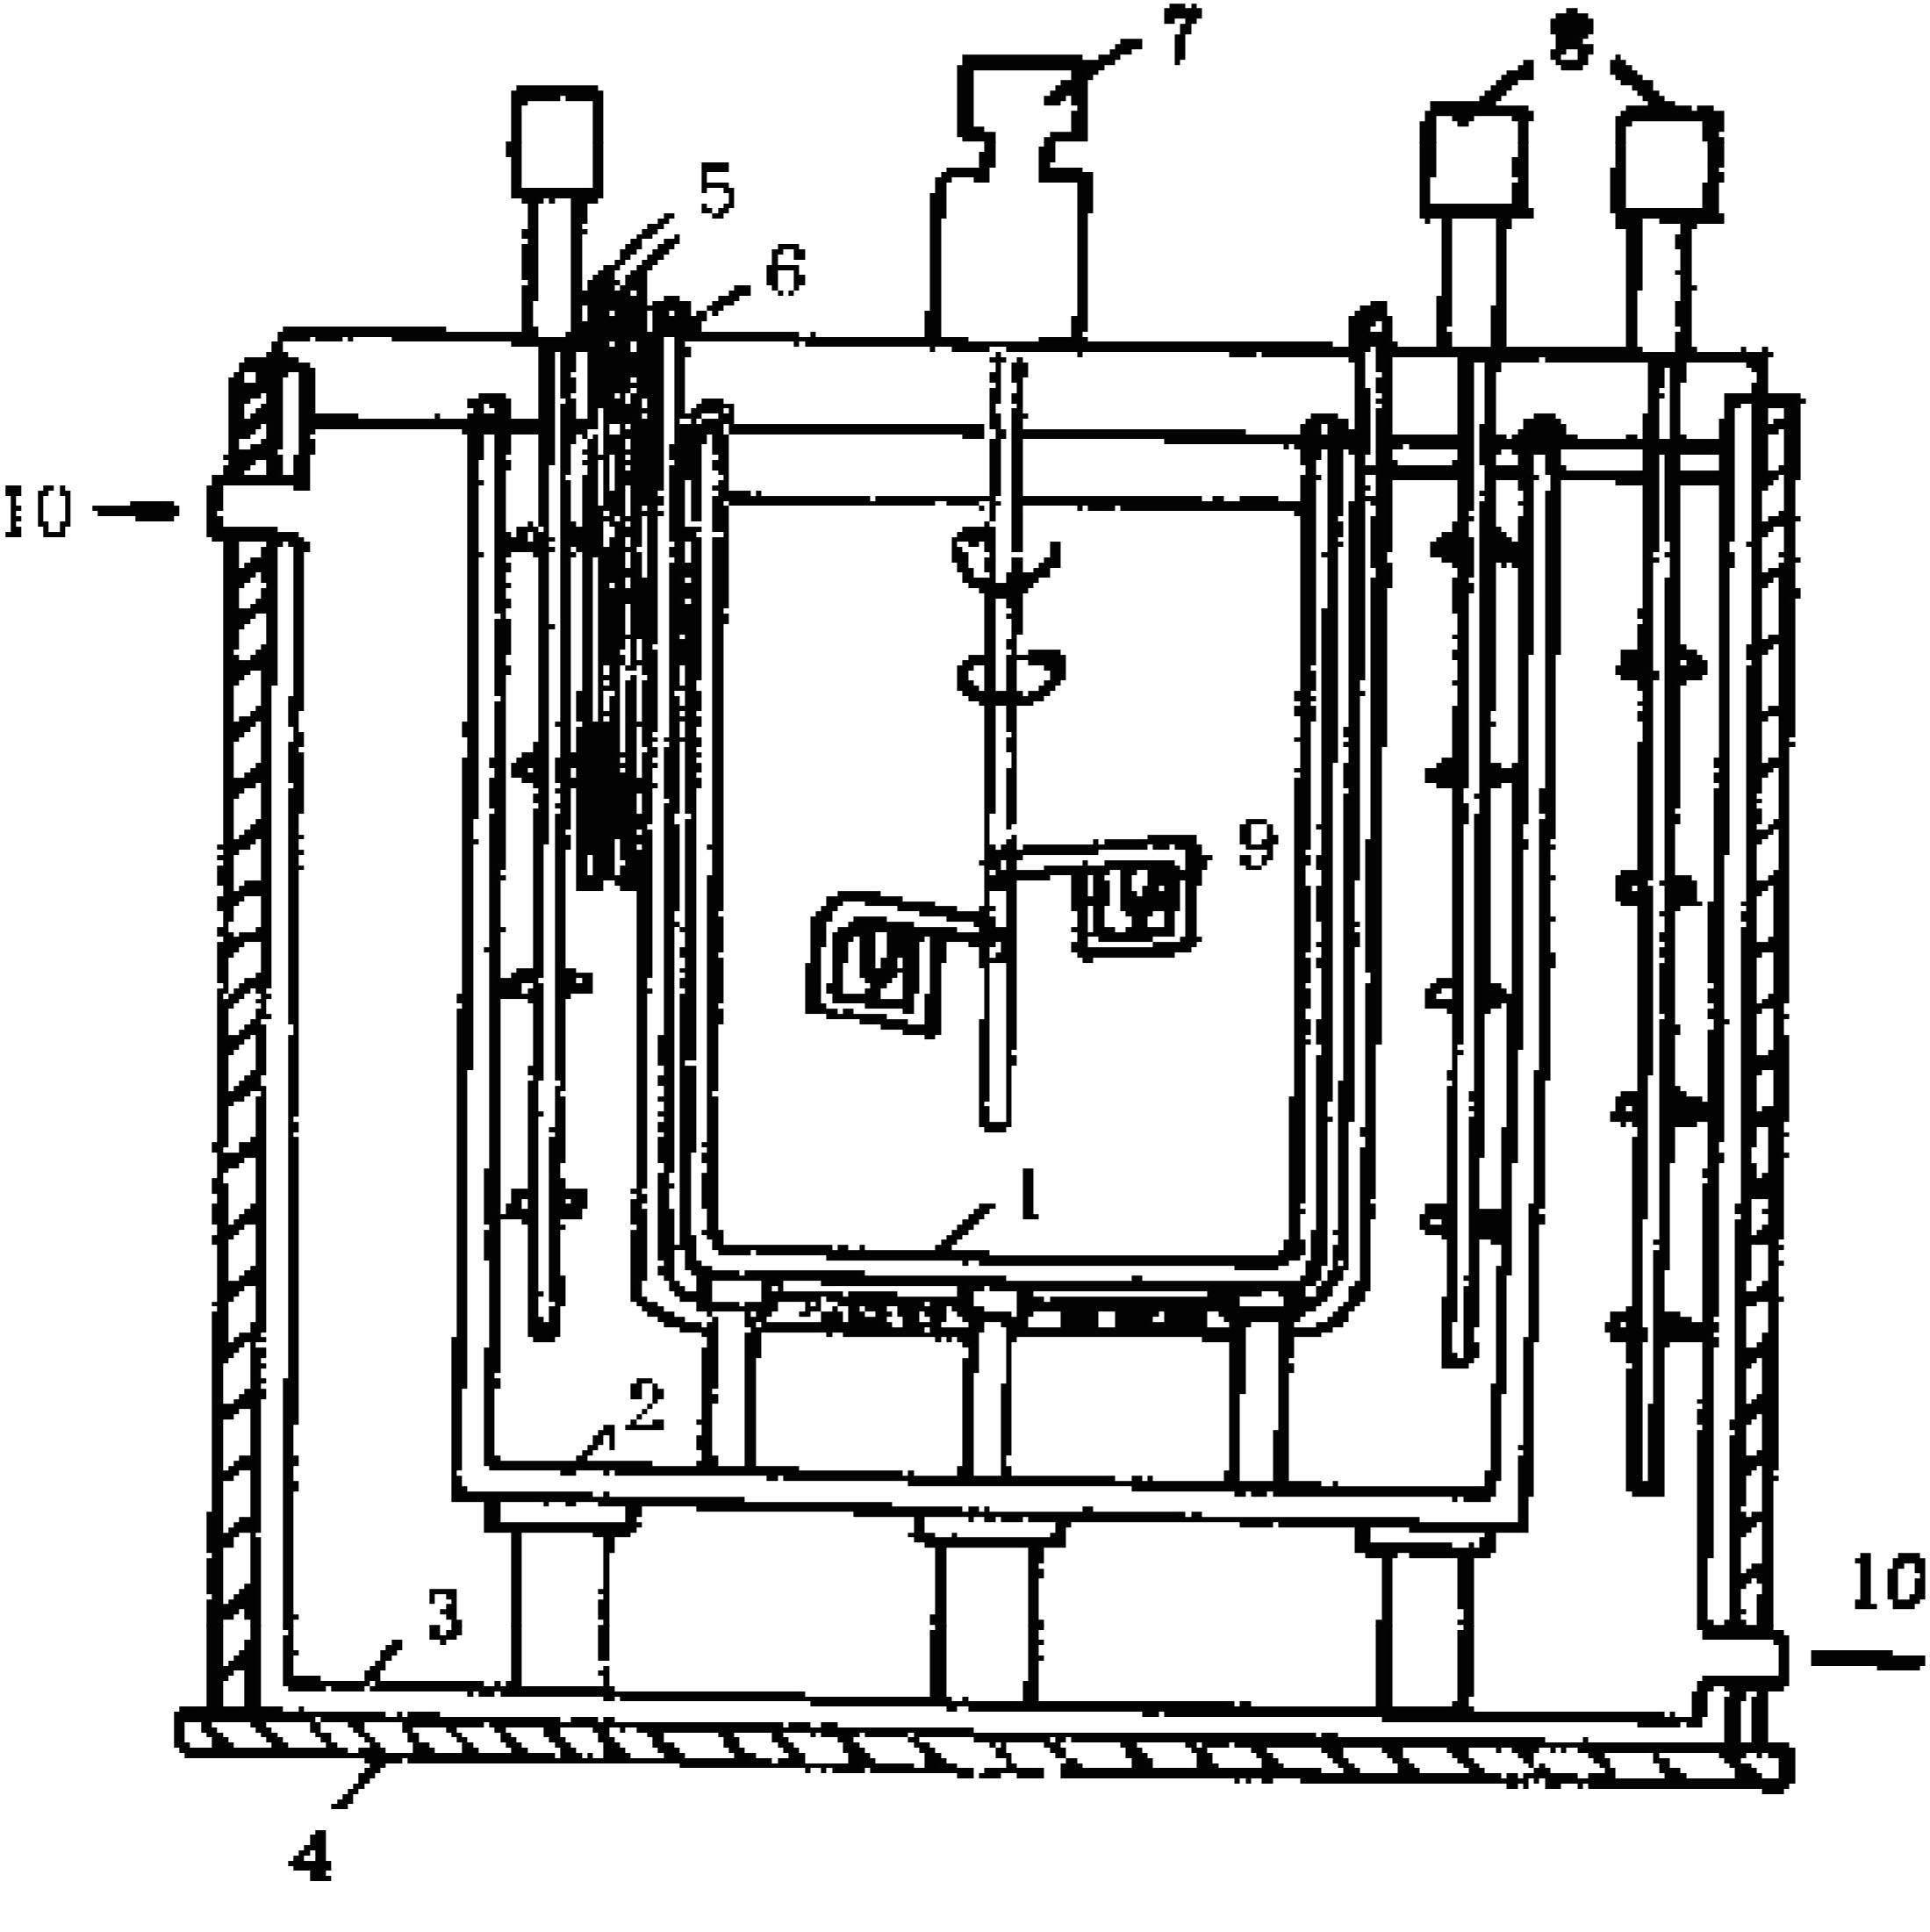
\includegraphics[width=0.45\textwidth]{fig/cp03/img3.20.jpg}
 \caption{双浴槽育晶装置。图中:}
 1为育晶器;2为内浴槽;3为外浴槽;4为保温层;5为感温元件;6为加热元件;7为转晶马达;8为搅拌马达(1500r/min);9为籽晶;10为外接冷却装置的进出口。
\end{figure}

为使溶液温度均匀,并使生长中的各个晶面在过饱和溶液中能得到均匀的溶质供应,要求晶体对溶液作相对运动。这种运动可采取多种形式,如晃动法(晶体固定不动,摇晃整个育晶器)、转晶法(晶体在溶液中作自转,公转或行星式转动)等,其中以晶体在溶液中自转或公转最为常用。为了克服这种方式所造成的的某些晶面迎液而动和使另一些晶面总是背向液流的缺点,转动需要定时换向,即用以下程序进行控制:正转---停转---反转---停转---正转。

降温法控制晶体生长的主要关键是掌握合适的降温速度。使溶液始终处于亚稳区内,并维持适宜的过饱和度,降温速度一般取决于以下述几个因素:
\begin{enumerate}[(1)]\itemsep -0.5ex
\item 晶体的最大透明生长速度(即在一定条件下不产生宏观缺陷的最大生长速度)。这一数值对不同晶体是有明显差别的(和亚稳区大小有关),例如对硝酸钠(NaNO$_3$)晶体为1mm/d,酒石酸钾钠(KNT)晶体则可达5mm/d以上。对同一晶体该数值还和晶体尺寸有关。
\item 溶解度的温度系数。溶解度的温度系数不但随不同物质而异,而且对同一种物质在不同的温度区间也一样。例如KDP的溶解度曲线在高温部分(50---70℃)温度系数较大,在低温部分(30℃以下)则较小。
\item 溶液的体积V(ml)和晶体生长表面积S(cm$^2$)之比,简称体面比。有些晶体(如KDP型晶体)在生长过程中,生长面积基本不变,而有些晶体(如KNT)在各个方向上都生长,S在生长过程中则在不断增加。
\end{enumerate}

总之,上述三个因素对于不同晶体是有明显差别的;对同一种晶体,这些因素在生长过程中也是在变化的。因此必须从实际出发,对不同的晶体在不同的阶段制定不同的降温程序。一般来说,在生长初期降温要慢,到了生长后期可稍快些。掌握规律后,可按程序实行自动降温。

必须指出,无宏观缺陷的晶体不一定是高质量的晶体(见3.4.3节)。培养用于光学目的高完整性的单晶,其生长速度应当控制的更小一些。

在控制降温过程中,最好能随时测定溶液的过饱和度(见3.1.4节)。同时,一些晶体生长现象[如生长涡流的强弱,晶面相对大小的变化,次要面的出现和消失,晶面花纹(见3.4.3节)等]往往是溶液过饱和度偏高或偏低以及晶体均匀性将遭破坏的“信号”。这些现象也可作为估计过饱和度、控制降温速度的参考信号。 %降温法
\subsection{流动法(温差法)}
流动法生长晶体装置一般由三部分组成(图3.21):生长槽(育晶器)C,溶解槽A和过热槽B。三槽之间的温度是B槽的温度高于A槽的温度高于A槽的,而A槽的温度又高于C槽的,A槽中过剩的原料在不断地搅拌下溶解,使溶液在高于C槽的温度在饱和,然后经过滤器进入过热槽B。过热槽的温度一般高于生长槽温度5--10℃。可以充分溶解从溶解槽流入的微晶,以提高溶液的稳定性。经过过热后的溶液用泵打入生长槽C,C槽的溶液是过饱和的,保证晶体生长有一定的驱动力。由于晶体的生长,从而使变稀的溶液流到溶解槽溶解原料,使溶液重新达到饱和,溶液如此循环流动,晶体不断生长。晶体的生长速度受到溶液的流动速度和A,C两槽温差的控制。这种方法的优点是生长温度和过饱和度都固定。使晶体始终在最有利的温度和最合适的过饱和度下生长,避免了因生长温度和过饱和度变化而产生的杂质分凝不均匀和生长带等缺陷,使晶体完整性更好。流动发的另一个优点就是生长大批量的晶体和培养大单净不收溶解度和溶液体积的影响,只受生长容器大小的限制。日本大阪大学用这种方法长出400$\times$400$\times$600mm大KDP晶体,生长速度达2mm/d。流动法的缺点是设备比较复杂,调节三槽之间适当的温度梯度和溶液流速之间的关系需要有一定的经验。
\begin{figure}[h]
 \centering
 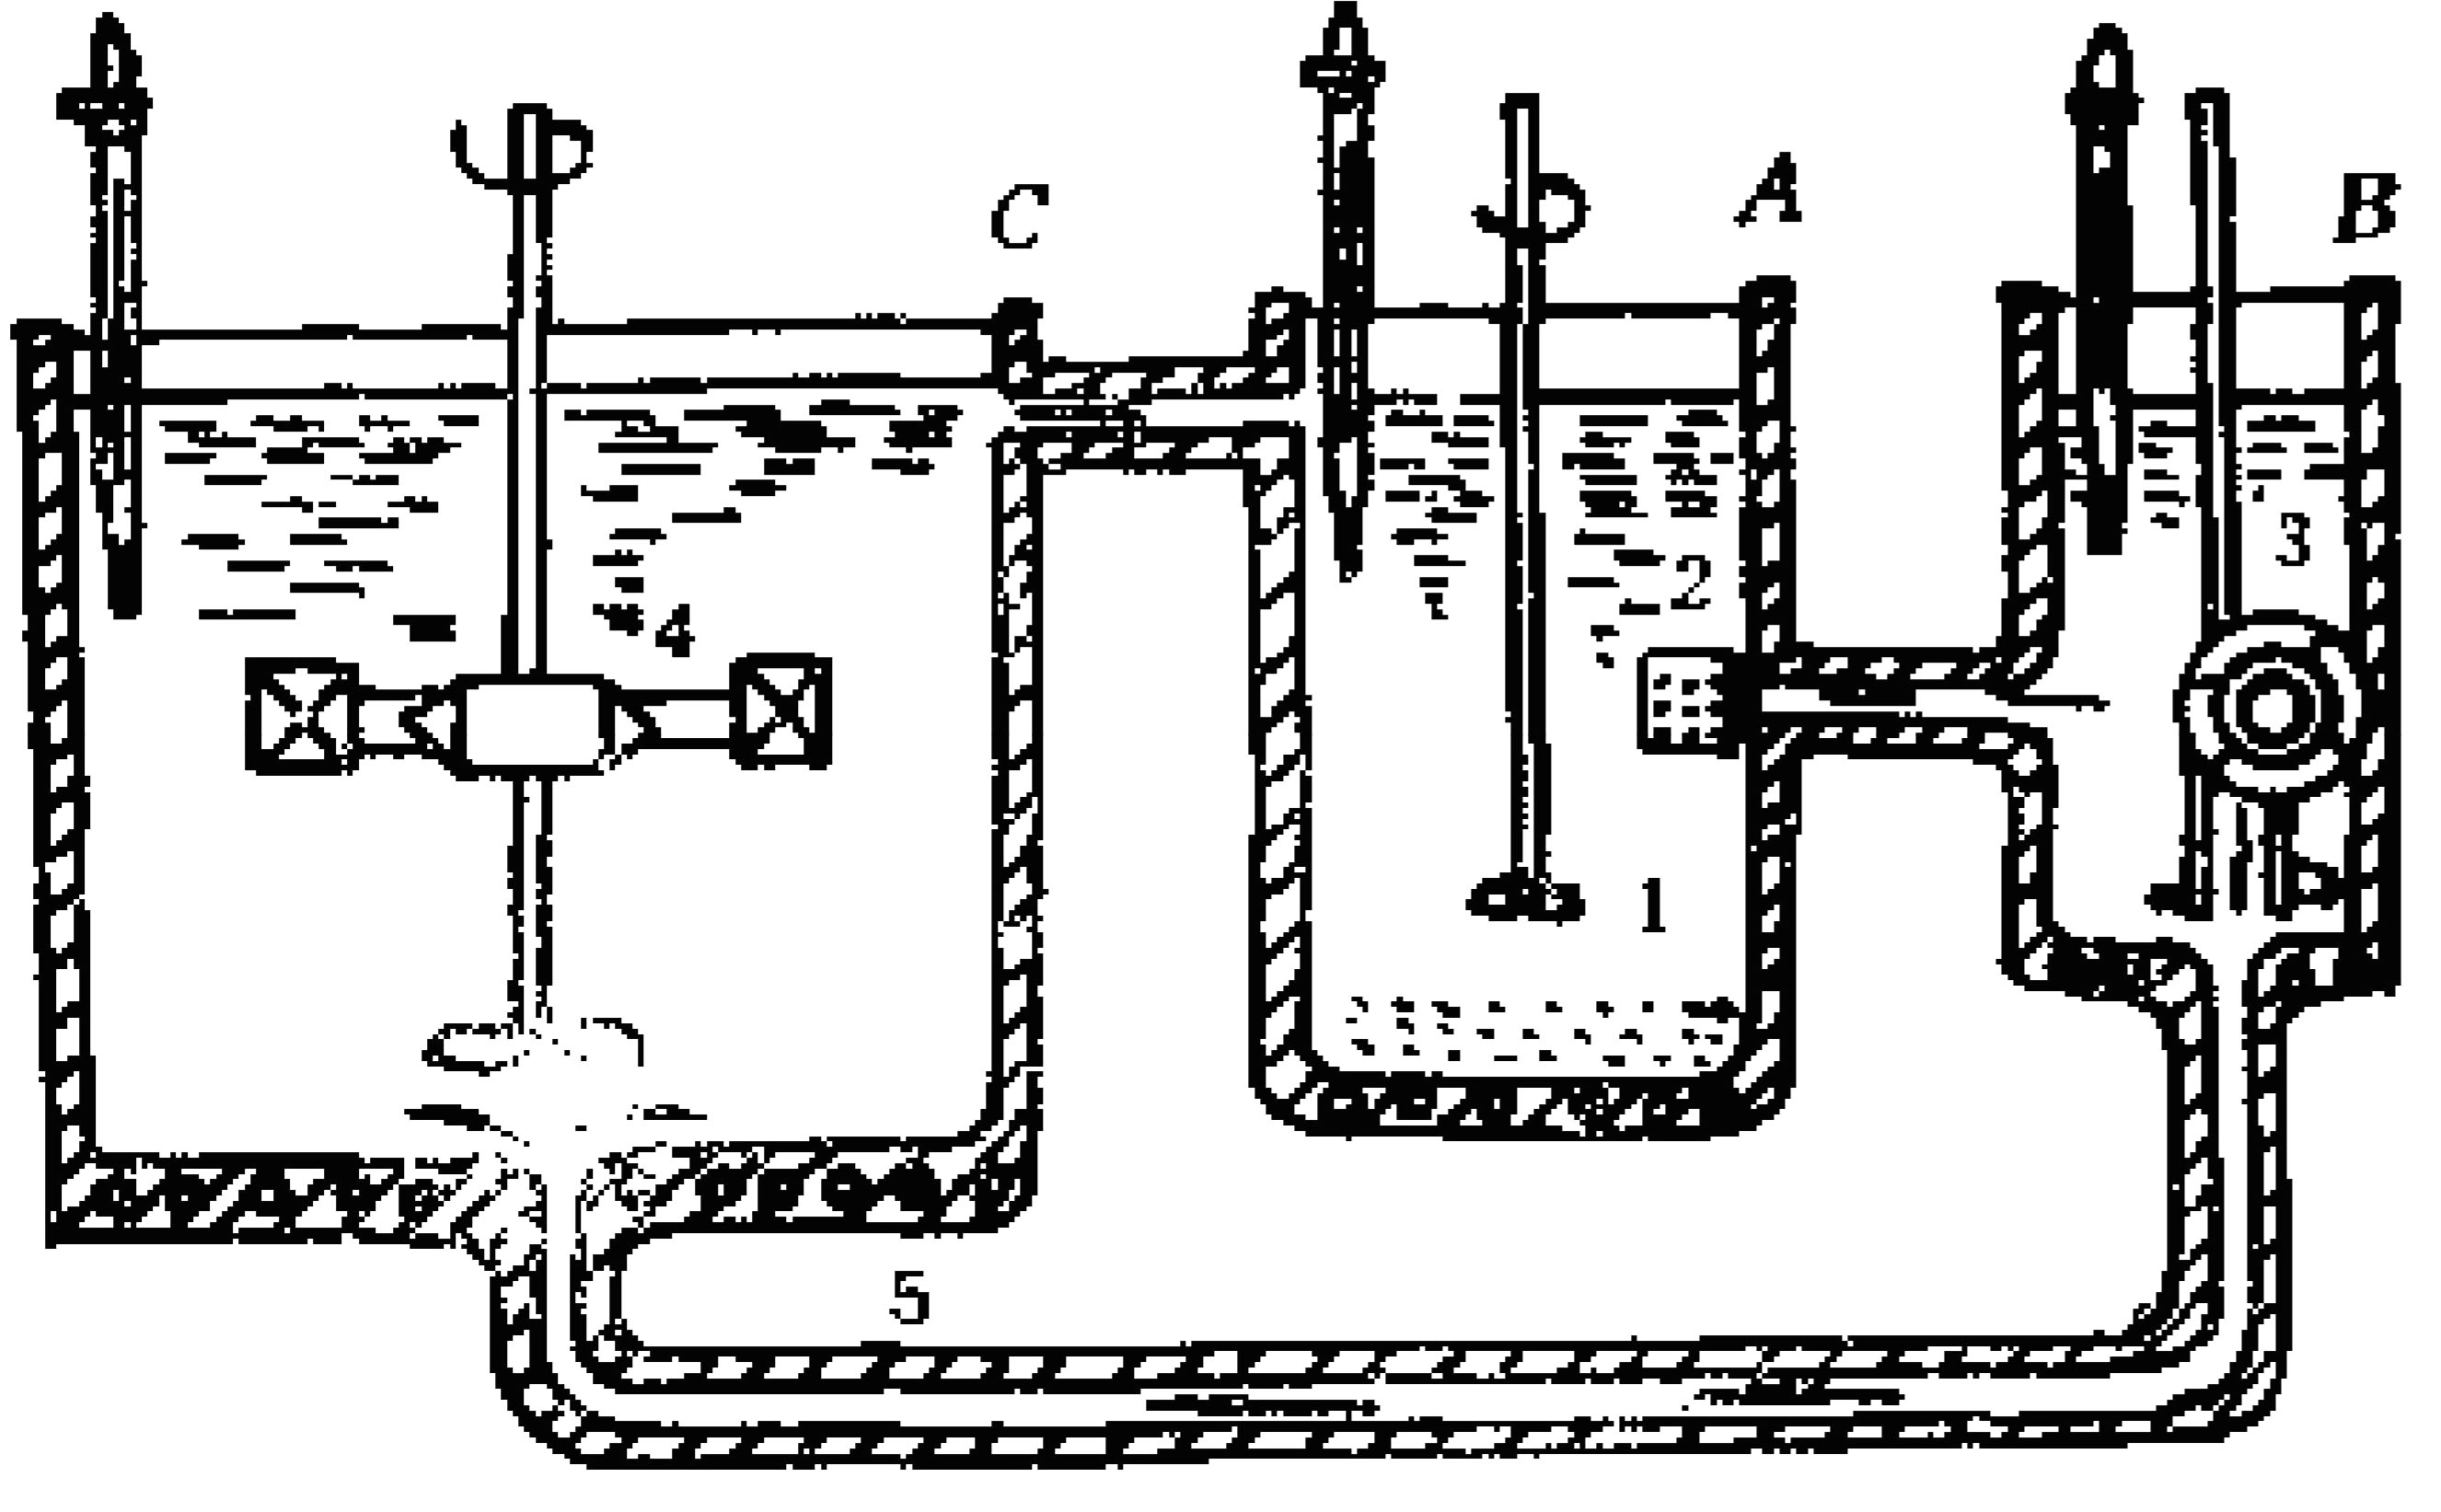
\includegraphics[width=0.6\textwidth]{fig/cp03/img3.21.jpg}
 \caption{循环流动育晶装置}
\end{figure}

采用适当装置也可以利用浓差自然对流来生长晶体。图3.22示出利用亚稳相和稳定相溶解度的差别通过浓差对流来生长$\alpha$-LiIO$_3$体的装置。两连通的玻璃槽,右边装$\beta$-LiIO$_3$原料,左边为生长槽,由于在20--30℃时,$\beta$-LiIO$_3$的溶解度比$\alpha$-LiIO$_3$的大1--2\%。浓度较大的LiIO$_3$溶液靠自然对流进入左边生长区,生长槽下部设置加热器,将溶液温度保持在40℃,造成对$\alpha$-LiIO$_3$的过饱和,析出的溶质在$\alpha$-LiIO$_3$种子上生长,变稀的溶液上升流回右边的原料槽重新溶解$\beta$-LiIO$_3$,原料槽靠空气冷却稳定在20--30℃。
\begin{figure}[h]
 \centering
 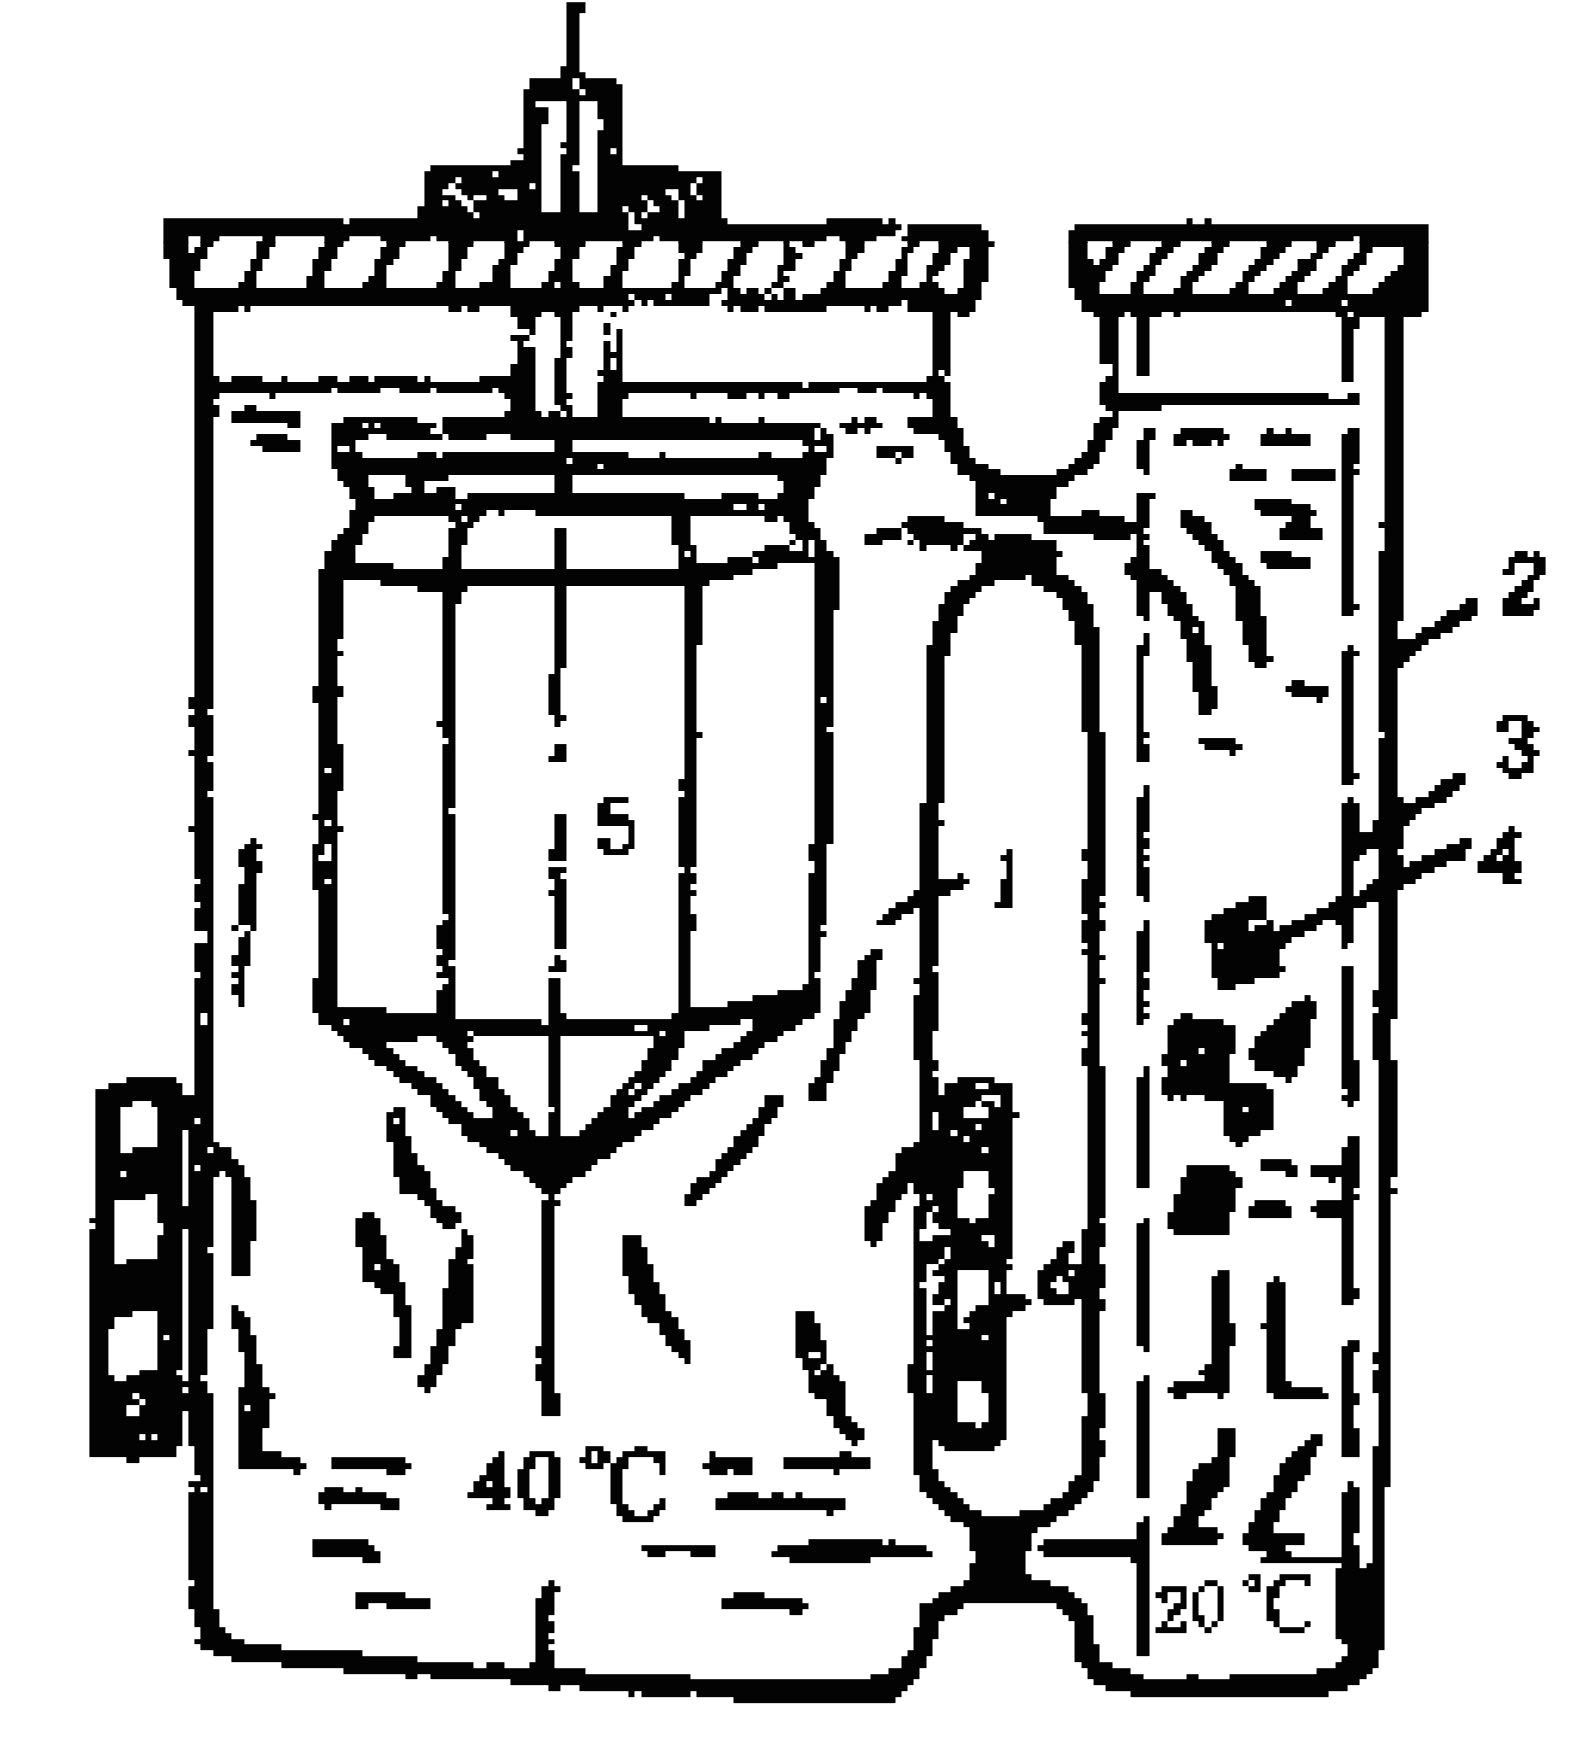
\includegraphics[width=0.5\textwidth]{fig/cp03/img3.22.jpg}
 \caption{浓差对流法生长LiIO$_3$晶体的装置}
\end{figure} %浓差法
\subsection{蒸发法}
蒸发法生长晶体的基本原理是将溶剂不断蒸发移去,而使溶液保持在过饱和状态,从而使晶体不断生长,这种方法比较适合于溶解度较大而其温度系数很小或是具有负温度系数的物质(表3.8)。蒸发法和流动法一样,晶体生长也是在恒温下进行的。不同是流动法用补充溶质,而蒸发法用移去溶剂来造成过饱和度。

蒸发法生长晶体的装置和降温法的装置十分类似。所不同的是在降温法中,育晶器中蒸发产生的冷凝水全部回流,而蒸发法则是部分回流。降温法通过降温速度来控制过饱和度,而蒸发法则是通过控制回流比(蒸发量)来控制过饱和度的。

\begin{table}[h]
\centering
\caption{一些适用于蒸发法生长的晶体在60℃时的溶解度及其温度系数}
\begin{tabular}{c|c|c}\toprule
物质 & \tabincell{c}{溶解度\\(g/1000g溶液)} & \tabincell{c}{溶解度温度系数\\g/1000g溶液$\cdot$℃}\\\hline
$\rm K_4HPO_4$ & 720 & $+0.1$\\
$\rm Li_2SO_4\cdot H_2O$ & 244 & $-0.36$\\
$\rm LiIO_3$ & 431 & $0.2$\\
\bottomrule
\end{tabular}
\end{table}

蒸发法生长晶体的装置有许多类型。图3.23示出的是比较简单的一种:在严格密封的育晶器上方设置冷凝器(可通水冷却)。溶剂自溶液表面不断蒸发,水蒸汽在冷凝器上凝结,并积聚在其下方的小杯内,再用虹吸管按控制量移出育晶器外,在晶体生长过程中,取水速度应小于冷凝速度,使大部分冷凝水(包括器壁上的)回流到液面上去,否则液面上易产生自发结晶。这种装置比较适合在较高的生长温度($>$60℃)使用。温度较低。蒸发量太小,不能满足晶体生长的需要。

\begin{figure}[htb]
 \centering
 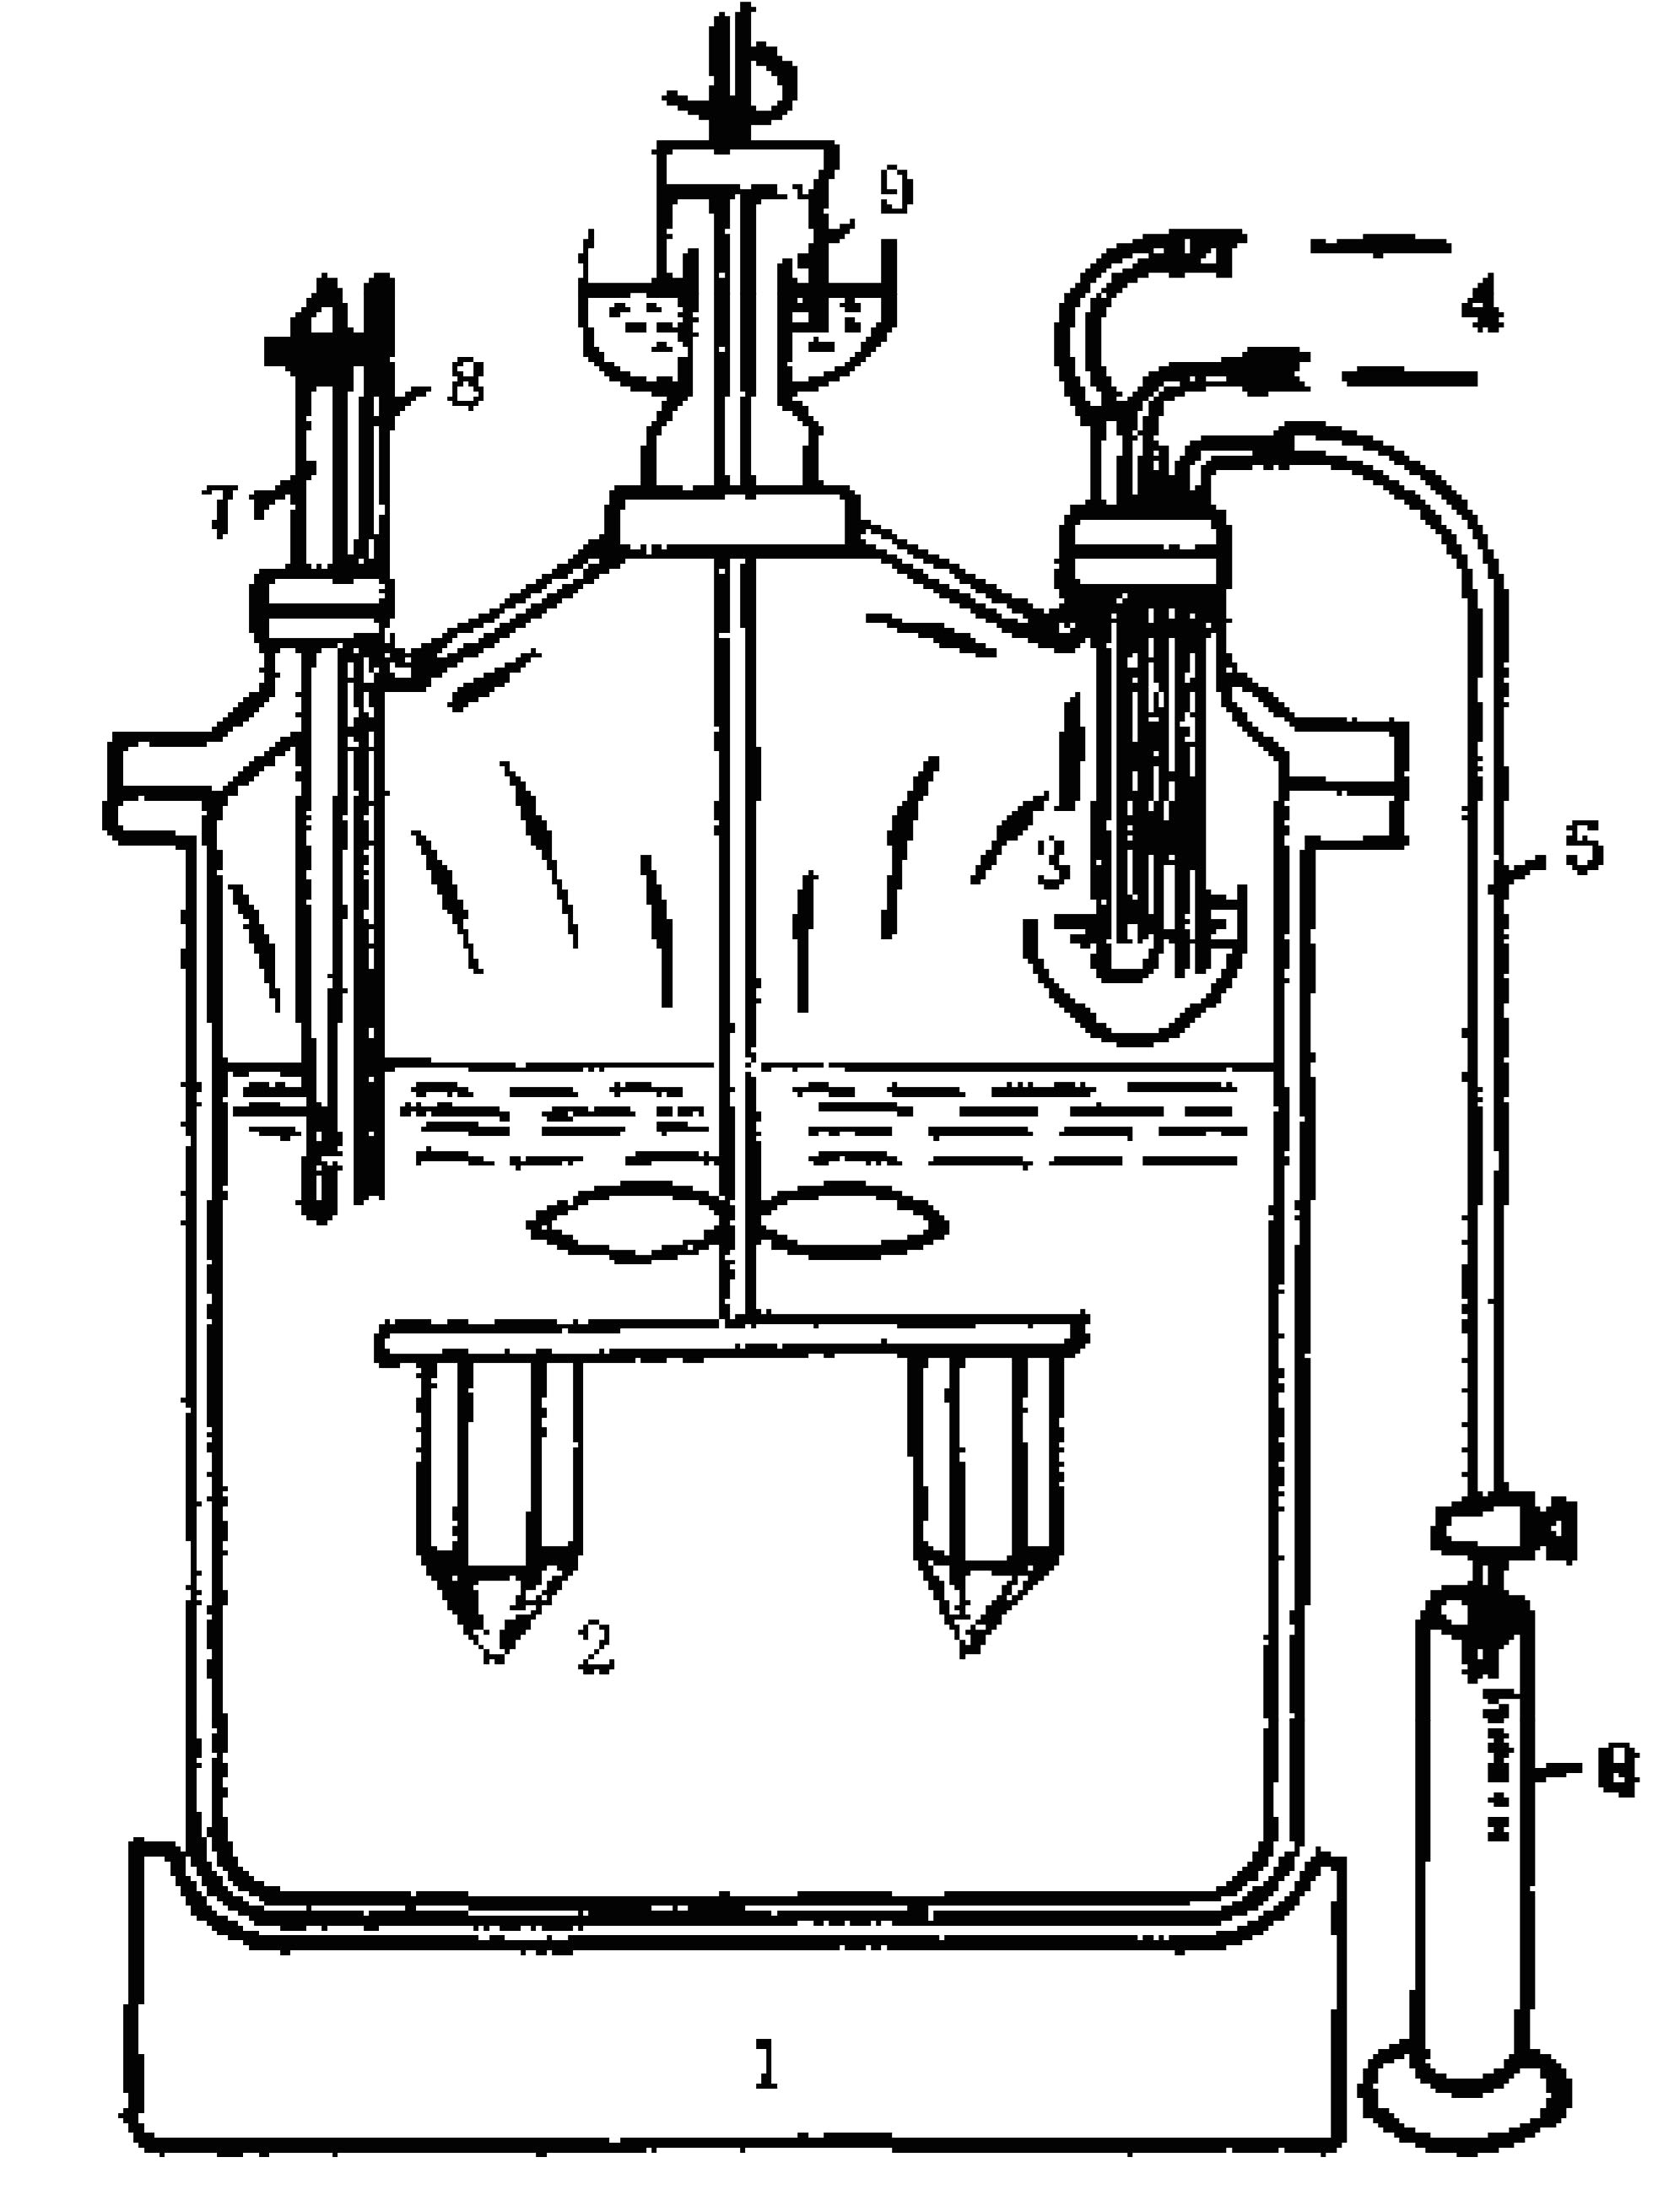
\includegraphics[width=0.4\textwidth]{fig/cp03/img3.23.jpg}
 \caption{蒸发法育晶装置。}
\end{figure}

\begin{figure}[hbt]
 \centering
 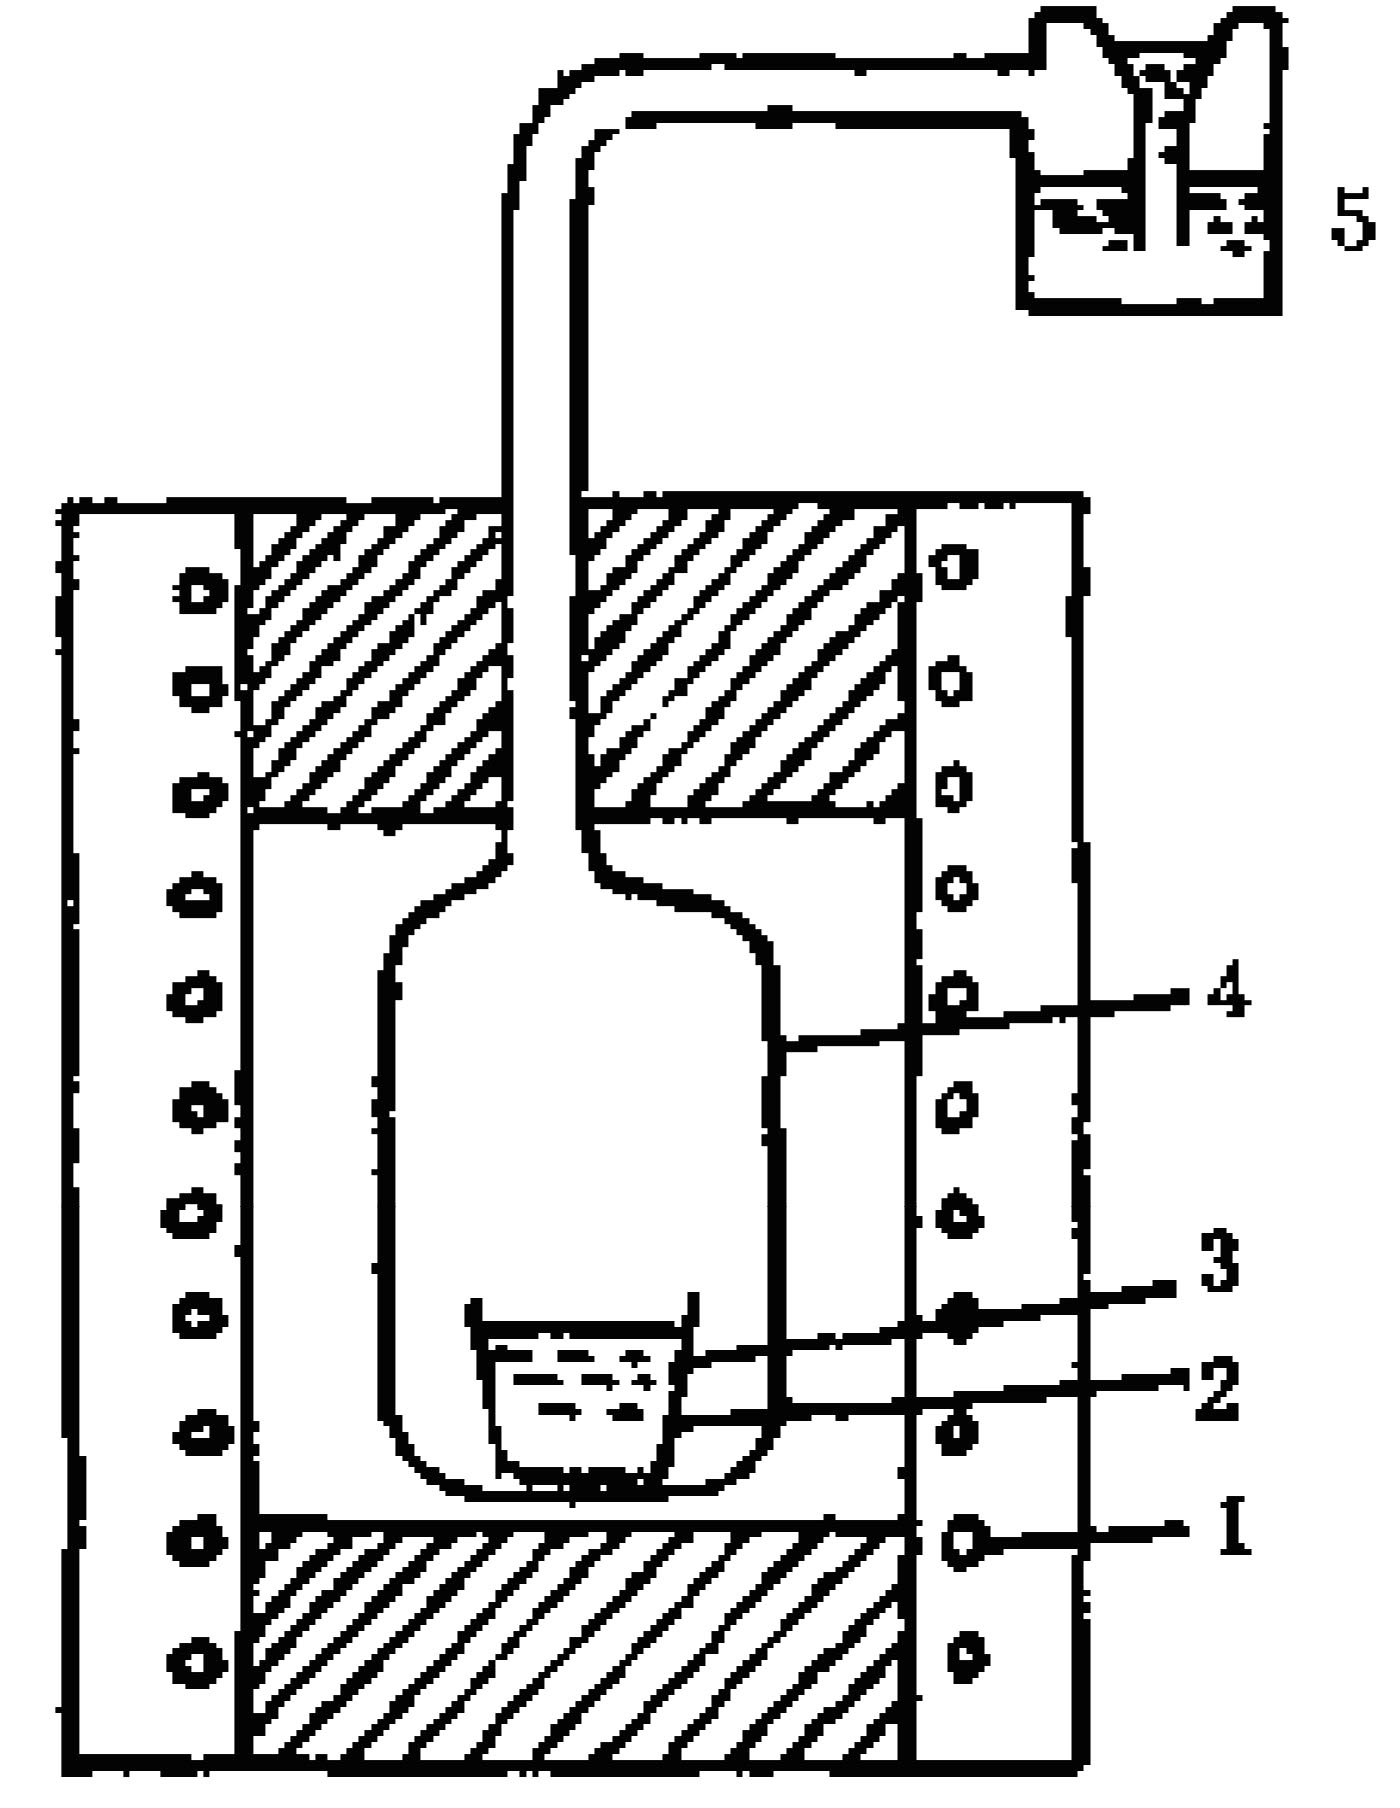
\includegraphics[width=0.4\textwidth]{fig/cp03/img3.24.jpg}
 \caption{生长NdPP晶体的装置。}
\end{figure}

有时体系中某一成分(如水)的蒸发并不是作为溶剂蒸发直接导致晶体生长,而是引起化学反应,间接导致晶体生长,例如在$\rm Nd_2O_3-H_3PO_4$(或$\rm Nd_2O_3-P_2O_5-H_2O$)体系中生长五磷酸钕($\rm NdP_5O_{14}$简称NdPP)晶体,其形成机制可能是
$$ \rm 14\ H_3PO_4 + Nd_2O_3 \xrightarrow{>260℃} 2\ NdP_5O_{14}+2\ H_4P_2O_7+17\ H_2O\uparrow$$

NdPP在焦磷酸($\rm H_4P_2O_7$)中有较大的溶解度,所以不会从溶液中析出,当温度升至300℃以上,焦磷酸逐渐脱水,形成多聚偏磷酸,NdPP在其中溶解度很小,在升温和蒸发过程中,由于焦磷酸浓度降低而使NdPP在溶液中到达过饱和而结晶出来
$$\rm n\ H_4P_2O_7 + NdP_5O_{14} \xrightarrow{>300℃} 2\ (HPO_3)_n + NdP_5O_{14}\downarrow + n\ H_2O\uparrow $$

据此机理,采用图3.24所示装置,在一定的温度下,控制水的蒸发速率就可以生长出质量较好的NdPP晶体。

这种晶体生长方式实际上是晶体在无机溶剂(焦磷酸)的溶液中,通过焦磷酸脱水蒸发而产生缩聚反应,使溶剂不断减少,并使溶质(NdPP)从其饱和溶液中结晶出来的过程。因此将其归入蒸发法。 %蒸发法
\subsection{电解溶剂法}
电解溶剂法是从溶液中生长晶体的一种独特的方法。其原理基于用电解法分解溶剂,以除去溶剂,使溶液处于过饱和状态。显然这种方法只能应用于溶剂可以被电解而其产物很容易自溶液中移去(如气体)的体系。同时还要求所培养的晶体在溶液中能导电而又不被电解。因此,这种方法特别适用于一些稳定的离子晶体的水溶液体系。

电解溶剂法的一半装置如图3.25所示。育晶器中装有铂电极,也起电解槽的作用,当通以稳定的直流电,溶剂就被电解,其速度由电流密度控制。溶液要搅拌以免产生浓差极化。溶液表面用流动液层(如邻二甲苯)覆盖以防溶剂蒸发,电解的产物从冷凝器中排除,在生长过程中,溶液pH应保持稳定。

\begin{figure}[h]
 \centering
 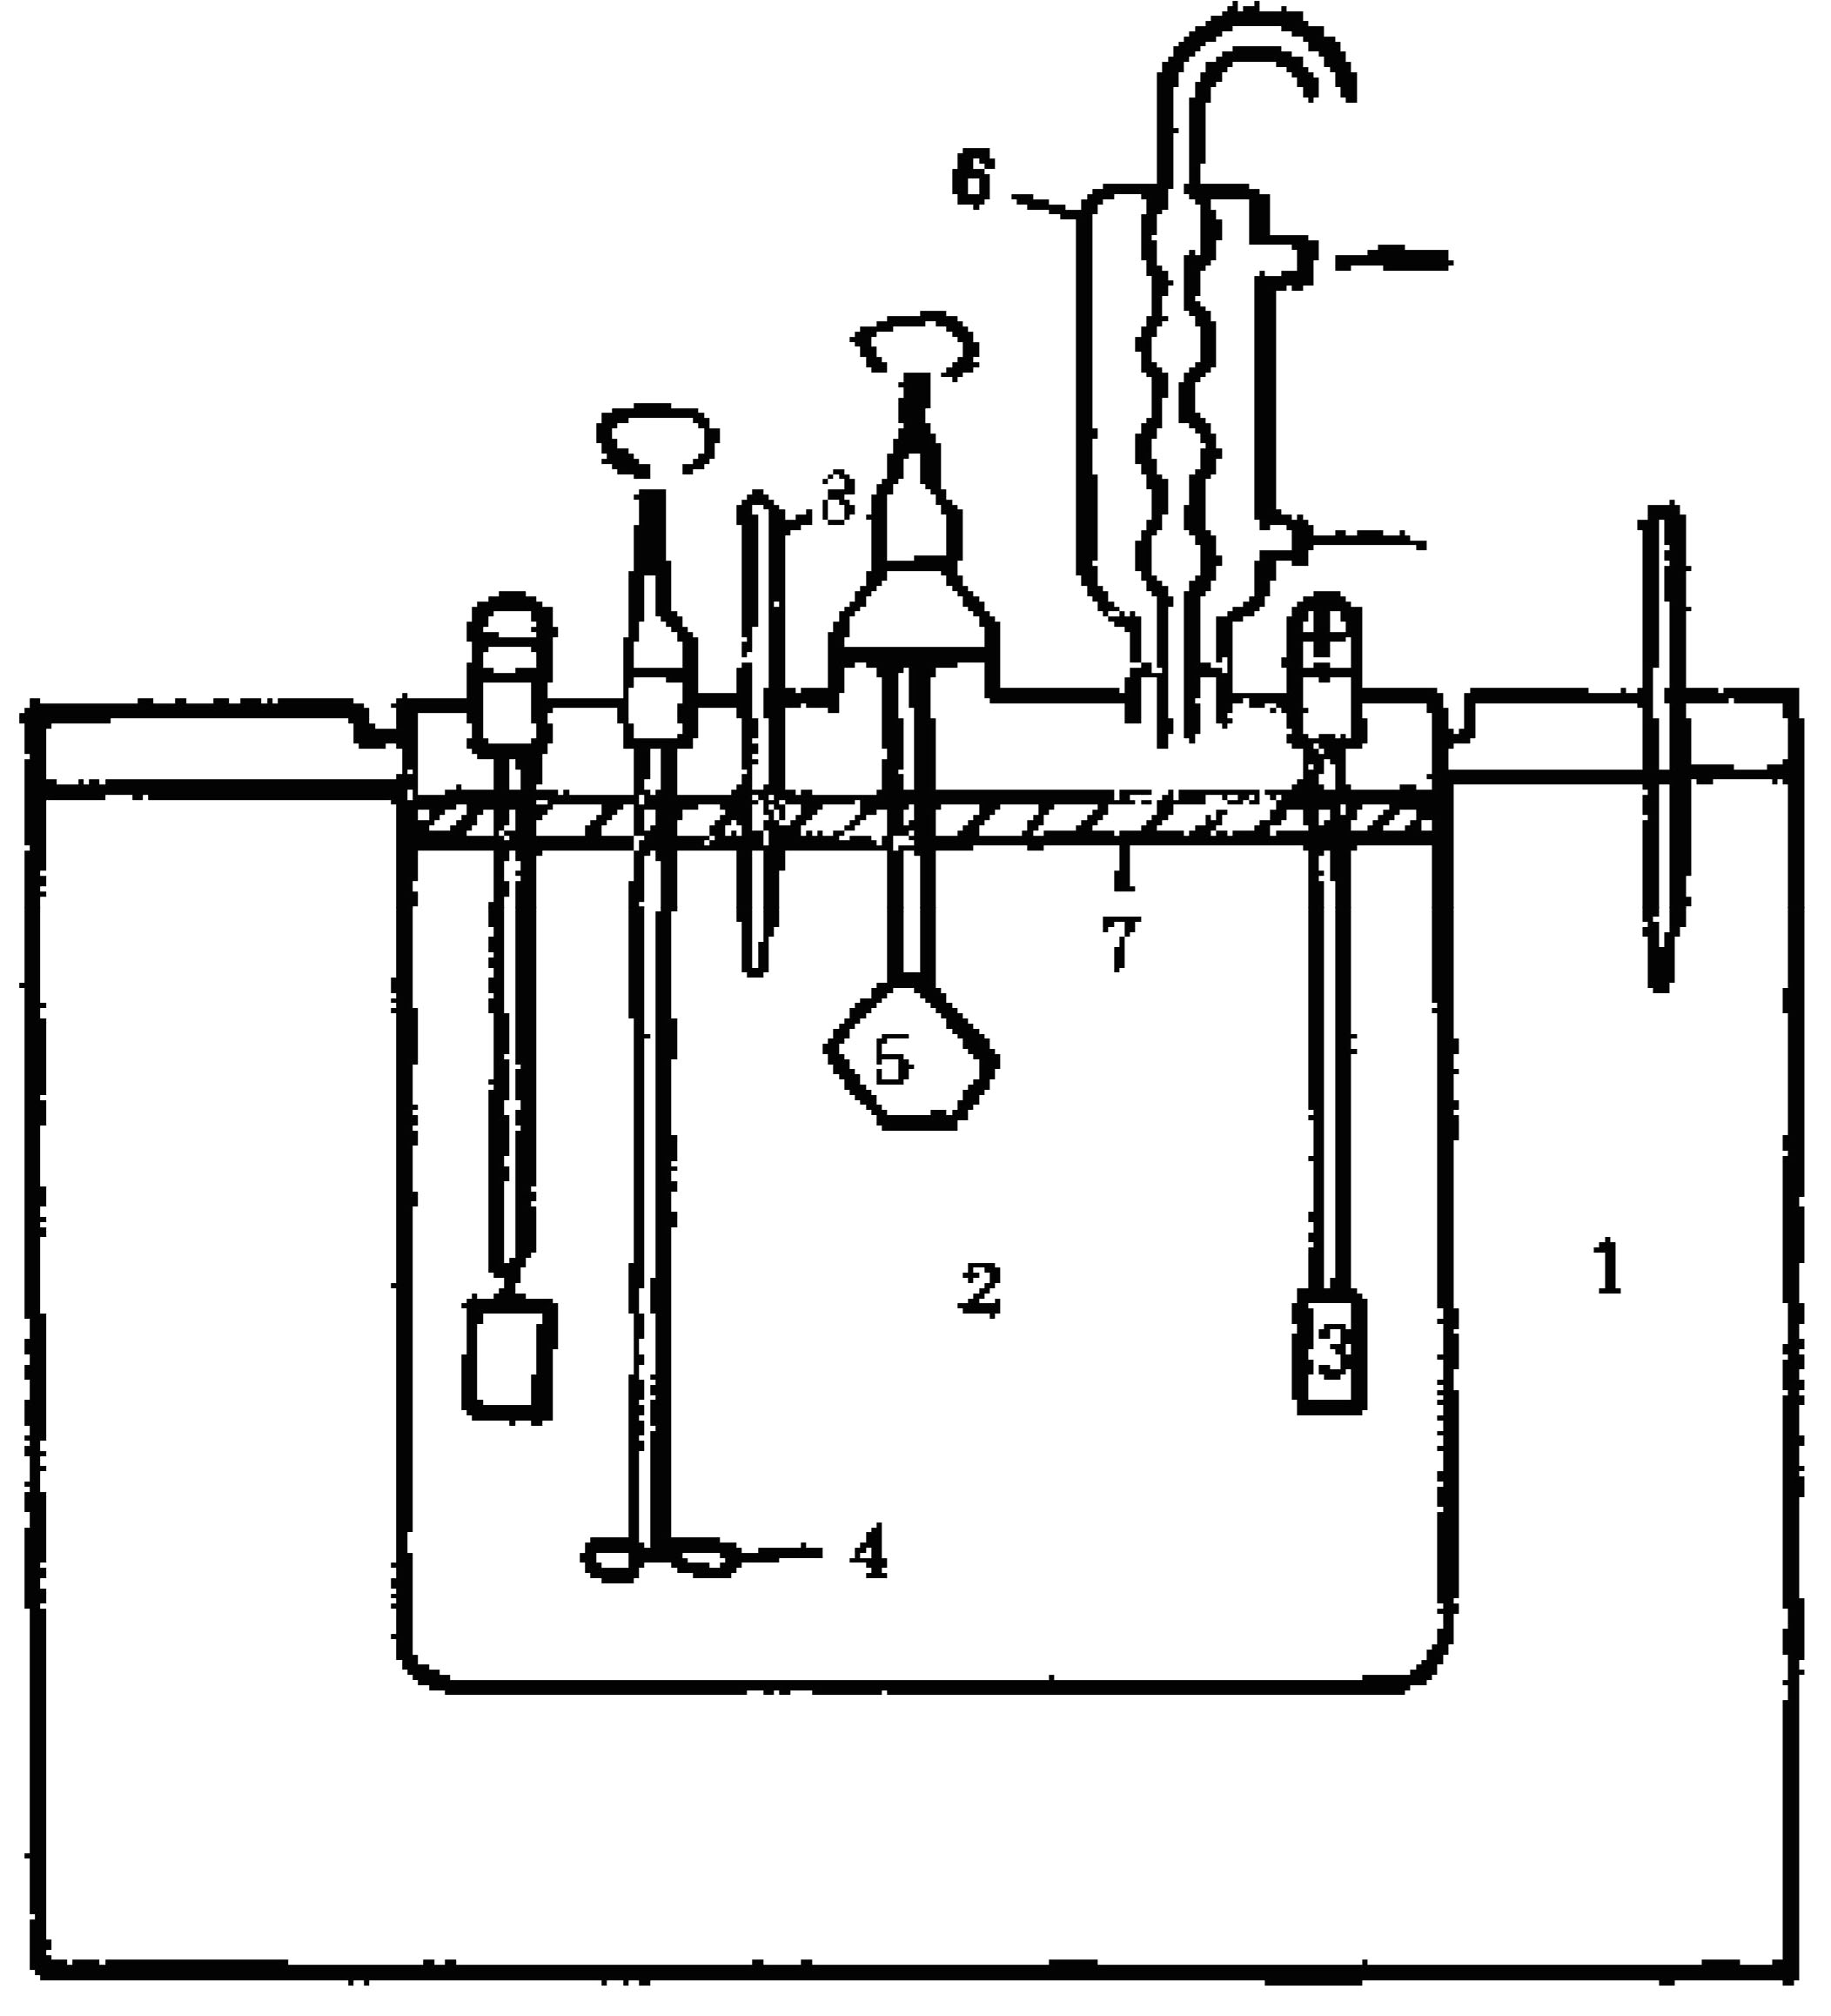
\includegraphics[width=0.5\textwidth]{fig/cp03/img3.25.jpg}
 \caption{电解溶剂法生长晶体装置图。}
\end{figure}

和流动法和蒸发法一样,用电解溶剂法生长晶体也是恒温下进行的。由于过饱和度使用直流电准确控制的,因此和生长温度关系不大,也可在室温下进行(这一点比蒸发法优越,因为温度较低时,蒸发量小,难以控制),也不需要知道溶解度曲线的情况。所以这种方法既适用于溶解度温度系数比较小的晶体,也适用于生长有数种晶相存在,而每种晶相仅在一定温度范围内才能稳定存在的晶体。

用电解溶剂法来生长KDP型(特别是DKDP晶体)获得了满意的结果。因为溶液中存在的常导致这些晶体柱面楔化的一些金属杂质离子(如Fe$^{3+}$,Al$^{3+}$,Cr$^{3+}$等)可以在电解过程中除去,从而消除这些杂质的有害影响。对DKDP晶体可以在低于其转变点的温度下生长,以防止单斜相的干扰,由于分解H$_2$O所需的能量比分解D$_2$O的要低,溶液中的H$_2$O在电解过程中比较容易除去。溶液在生长过程中可以保持较高的氘化程度。图3.26示出在普通转晶育晶器(图3.18)基础上改装的电解溶剂法生长这一类晶体的装置。阳极置于育晶器底部,为使电流均匀通过溶液,在溶液上方安置了两个电极,阴极放在喇叭形口的塑料管内,口上用尼龙网覆盖,使在阴极上产生的氢气引入通风良好的空间,防止其重新进入溶液。在阳极上产生的氧气进入育晶器中溶液上方的空间,保持正压,它投注于减少大气中的水汽和溶液中的氘发生交换而降低其含氘量。由于电解交流也会产生热量,因此也可以不使用底部加热器,而是将交流电直接通过电极加热,使用交、直流并用的加热—电解联合控制装置。晶体在溶液中转动以使溶液浓度均匀。由于溶液是强缓冲溶液,所以电解过程中溶液pH变化不大。

\begin{figure}[htbp]
 \centering
 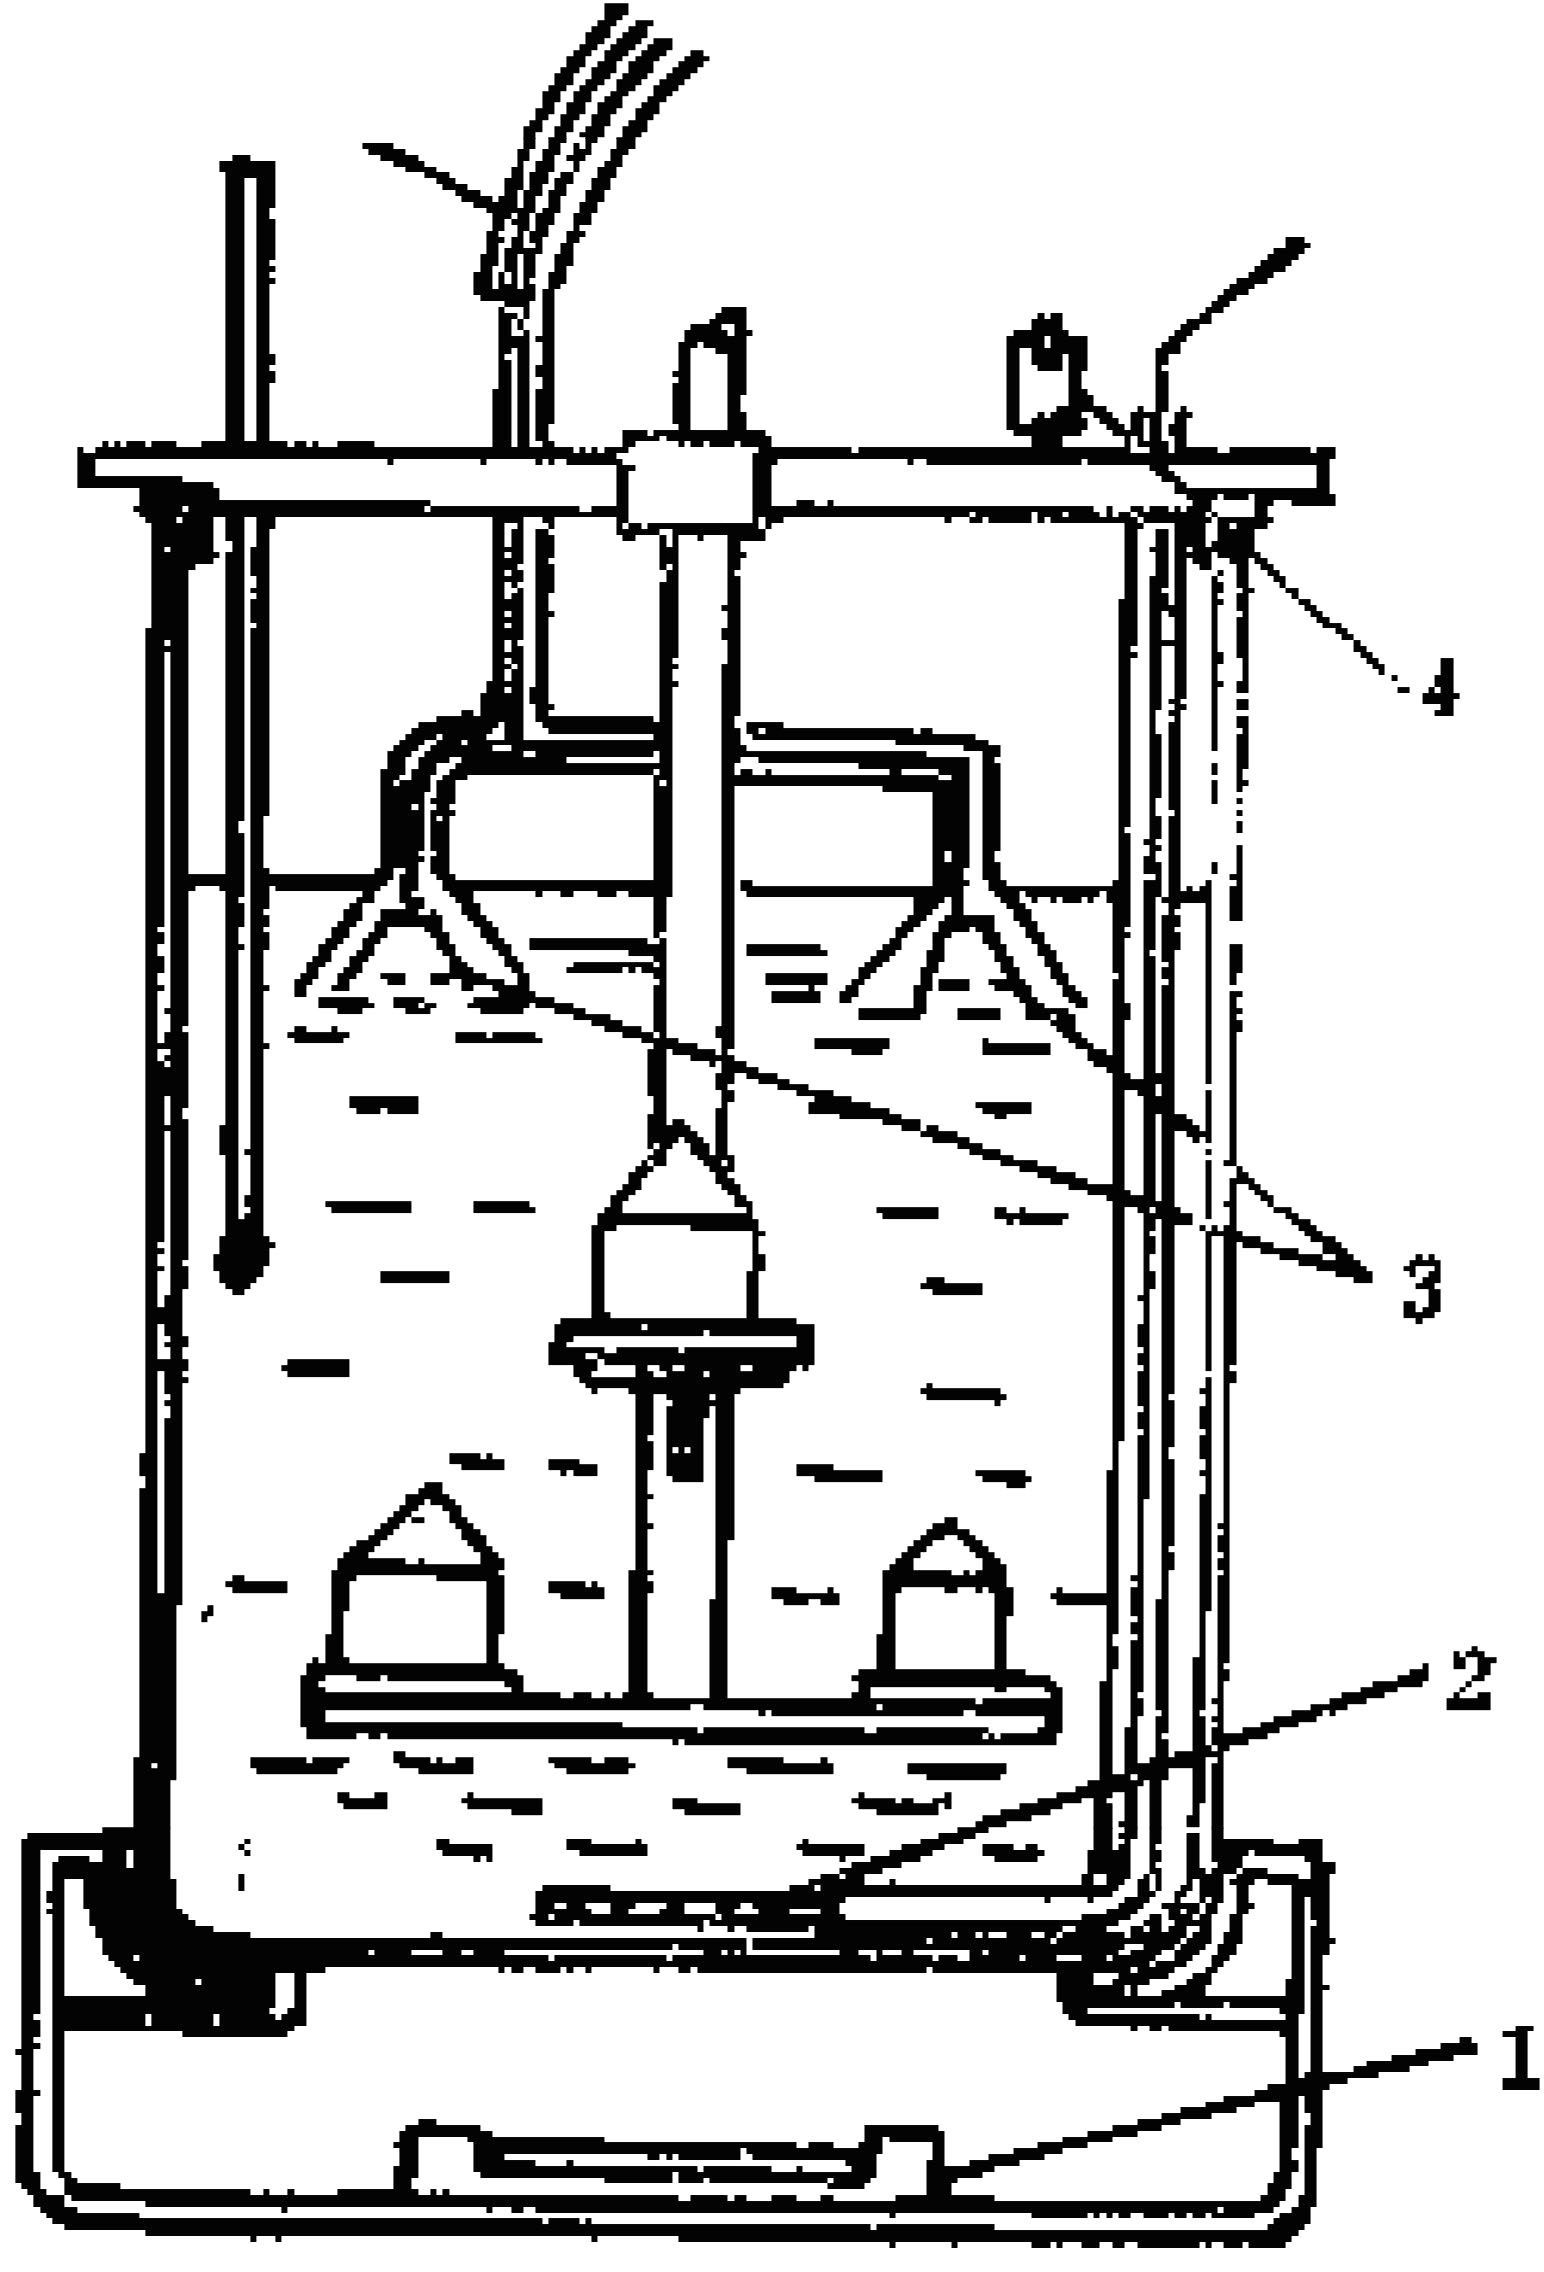
\includegraphics[width=0.4\textwidth]{fig/cp03/img3.26.jpg}
 \caption{由通常转晶育晶器改装的电解溶剂育晶装置。}
\end{figure}

对于从重水溶液中生长高质量的KDP型晶体,电解溶剂法是一种有前途的方法。

除了上述四种从水溶液中生长晶体的方法外,还有凝胶法,有机溶剂法等,这些内容将在下面独立的章节中进行论述。

上述的从溶液中生长晶体的各种方法中,以降温法、蒸发法、流动法最为常用,大部分水溶性晶体都是用这些方法培养的。表3.9列出了从溶液中生长的一些晶体的单晶培养和一般的结晶方法。

(表3.9  从溶液中生长的一些重要晶体)

 %电解溶剂法
